% Template for PLoS
% Version 3.5 March 2018
%
% % % % % % % % % % % % % % % % % % % % % %
%
% -- IMPORTANT NOTE
%
% This template contains comments intended
% to minimize problems and delays during our production
% process. Please follow the template instructions
% whenever possible.
%
% % % % % % % % % % % % % % % % % % % % % % %
%
% Once your paper is accepted for publication,
% PLEASE REMOVE ALL TRACKED CHANGES in this file
% and leave only the final text of your manuscript.
% PLOS recommends the use of latexdiff to track changes during review, as this will help to maintain a clean tex file.
% Visit https://www.ctan.org/pkg/latexdiff?lang=en for info or contact us at latex@plos.org.
%
%
% There are no restrictions on package use within the LaTeX files except that
% no packages listed in the template may be deleted.
%
% Please do not include colors or graphics in the text.
%
% The manuscript LaTeX source should be contained within a single file (do not use \input, \externaldocument, or similar commands).
%
% % % % % % % % % % % % % % % % % % % % % % %
%
% -- FIGURES AND TABLES
%
% Please include tables/figure captions directly after the paragraph where they are first cited in the text.
%
% DO NOT INCLUDE GRAPHICS IN YOUR MANUSCRIPT
% - Figures should be uploaded separately from your manuscript file.
% - Figures generated using LaTeX should be extracted and removed from the PDF before submission.
% - Figures containing multiple panels/subfigures must be combined into one image file before submission.
% For figure citations, please use "Fig" instead of "Figure".
% See http://journals.plos.org/plosone/s/figures for PLOS figure guidelines.
%
% Tables should be cell-based and may not contain:
% - spacing/line breaks within cells to alter layout or alignment
% - do not nest tabular environments (no tabular environments within tabular environments)
% - no graphics or colored text (cell background color/shading OK)
% See http://journals.plos.org/plosone/s/tables for table guidelines.
%
% For tables that exceed the width of the text column, use the adjustwidth environment as illustrated in the example table in text below.
%
% % % % % % % % % % % % % % % % % % % % % % % %
%
% -- EQUATIONS, MATH SYMBOLS, SUBSCRIPTS, AND SUPERSCRIPTS
%
% IMPORTANT
% Below are a few tips to help format your equations and other special characters according to our specifications. For more tips to help reduce the possibility of formatting errors during conversion, please see our LaTeX guidelines at http://journals.plos.org/plosone/s/latex
%
% For inline equations, please be sure to include all portions of an equation in the math environment.  For example, x$^2$ is incorrect; this should be formatted as $x^2$ (or $\mathrm{x}^2$ if the romanized font is desired).
%
% Do not include text that is not math in the math environment. For example, CO2 should be written as CO\textsubscript{2} instead of CO$_2$.
%
% Please add line breaks to long display equations when possible in order to fit size of the column.
%
% For inline equations, please do not include punctuation (commas, etc) within the math environment unless this is part of the equation.
%
% When adding superscript or subscripts outside of brackets/braces, please group using {}.  For example, change "[U(D,E,\gamma)]^2" to "{[U(D,E,\gamma)]}^2".
%
% Do not use \cal for caligraphic font.  Instead, use \mathcal{}
%
% % % % % % % % % % % % % % % % % % % % % % % %
%
% Please contact latex@plos.org with any questions.
%
% % % % % % % % % % % % % % % % % % % % % % % %

\documentclass[10pt,letterpaper]{article}
\usepackage[top=0.85in,left=2.75in,footskip=0.75in]{geometry}

% amsmath and amssymb packages, useful for mathematical formulas and symbols
\usepackage{amsmath,amssymb}

% Use adjustwidth environment to exceed column width (see example table in text)
\usepackage{changepage}

% Use Unicode characters when possible
\usepackage[utf8x]{inputenc}

% textcomp package and marvosym package for additional characters
\usepackage{textcomp,marvosym}

% cite package, to clean up citations in the main text. Do not remove.
\usepackage{cite}

% Use nameref to cite supporting information files (see Supporting Information section for more info)
\usepackage{nameref,hyperref}

% line numbers
\usepackage[right]{lineno}

% ligatures disabled
\usepackage{microtype}
\DisableLigatures[f]{encoding = *, family = * }

% color can be used to apply background shading to table cells only
\usepackage[table]{xcolor}

% array package and thick rules for tables
\usepackage{array}

\usepackage{booktabs}
\usepackage{tabularx}
\usepackage{caption}
\usepackage{subcaption}
\usepackage{placeins}

\captionsetup{compatibility=false}

% create "+" rule type for thick vertical lines
\newcolumntype{+}{!{\vrule width 2pt}}

% create \thickcline for thick horizontal lines of variable length
\newlength\savedwidth
\newcommand\thickcline[1]{%
  \noalign{\global\savedwidth\arrayrulewidth\global\arrayrulewidth 2pt}%
  \cline{#1}%
  \noalign{\vskip\arrayrulewidth}%
  \noalign{\global\arrayrulewidth\savedwidth}%
}

% \thickhline command for thick horizontal lines that span the table
\newcommand\thickhline{\noalign{\global\savedwidth\arrayrulewidth\global\arrayrulewidth 2pt}%
\hline
\noalign{\global\arrayrulewidth\savedwidth}}


% Remove comment for double spacing
%\usepackage{setspace}
%\doublespacing

% Text layout
\raggedright
\setlength{\parindent}{0.5cm}
\textwidth 5.25in
\textheight 8.75in

% Bold the 'Figure #' in the caption and separate it from the title/caption with a period
% Captions will be left justified
\usepackage[aboveskip=1pt,labelfont=bf,labelsep=period,justification=raggedright,singlelinecheck=off]{caption}
\renewcommand{\figurename}{Fig}

% Use the PLoS provided BiBTeX style
\bibliographystyle{plos2015}

% Remove brackets from numbering in List of References
\makeatletter
\renewcommand{\@biblabel}[1]{\quad#1.}
\makeatother


% Header and Footer with logo
\usepackage{lastpage,fancyhdr,graphicx}
\usepackage{epstopdf}
%\pagestyle{myheadings}
\pagestyle{fancy}
\fancyhf{}
%\setlength{\headheight}{27.023pt}
%\lhead{\includegraphics[width=2.0in]{PLOS-submission.eps}}
\rfoot{\thepage/\pageref{LastPage}}
\renewcommand{\headrulewidth}{0pt}
\renewcommand{\footrule}{\hrule height 2pt \vspace{2mm}}
\fancyheadoffset[L]{2.25in}
\fancyfootoffset[L]{2.25in}
\lfoot{\today}

%% Include all macros below

\newcommand{\lorem}{{\bf LOREM}}
\newcommand{\ipsum}{{\bf IPSUM}}

\newcolumntype{L}[1]{>{\raggedright\arraybackslash}p{#1}}
\newcolumntype{C}[1]{>{\centering\arraybackslash}p{#1}}
\newcolumntype{R}[1]{>{\raggedleft\arraybackslash}p{#1}}

%% END MACROS SECTION


\begin{document}
\vspace*{0.2in}

% Title must be 250 characters or less.
\begin{flushleft}
{\Large
\textbf\newline{Hydra: A mixture modeling framework for subtyping pediatric cancer cohorts using multimodal gene expression signatures} % Please use "sentence case" for title and headings (capitalize only the first word in a title (or heading), the first word in a subtitle (or subheading), and any proper nouns).
}
\newline
% Insert author names, affiliations and corresponding author email (do not include titles, positions, or degrees).
\\
Jacob Pfeil\textsuperscript{1,2*},
Lauren M. Sanders\textsuperscript{1,2,3},
Ioannis Anastopoulos\textsuperscript{1,2},
A. Geoffrey Lyle\textsuperscript{2,3},
Alana S. Weinstein\textsuperscript{1,2},
Yuanqing Xue\textsuperscript{1,2},
Andrew Blair\textsuperscript{1,2},
Holly C. Beale\textsuperscript{2,3},
Alex Lee\textsuperscript{4},
Stanley G. Leung\textsuperscript{4},
Phuong T. Dinh\textsuperscript{4},
Avanthi Tayi Shah\textsuperscript{4},
Marcus R. Breese\textsuperscript{4},
W. Patrick Devine\textsuperscript{5},
Isabel Bjork\textsuperscript{2},
Sofie R. Salama\textsuperscript{1,2,6\ddag},
E. Alejandro Sweet-Cordero\textsuperscript{4\ddag},
David Haussler\textsuperscript{1,2,6\ddag},
Olena Morozova Vaske\textsuperscript{2,3\ddag}
\\
\bigskip
\textbf{1} Department of Biomolecular Engineering, University of California, Santa Cruz, California, United States of America
\\
\textbf{2} Genomics Institute, University of California, Santa Cruz, California, United States of America
\\
\textbf{3} Department of Molecular, Cell and Developmental Biology, University of California, Santa Cruz, California, United States of America
\\
\textbf{4} Department of Pediatrics, Division of Hematology and Oncology, University of California, San Francisco, California, United States of America
\\
\textbf{5} Department of Anatomic Pathology, University of California, San Francisco, California, United States of America
\\
\textbf{6} Howard Hughes Medical Institute, University of California, Santa Cruz, California, United States of America
\\
\bigskip
%\textbf{1000} Affiliation Dept/Program/Center, Institution Name, City, State, Country

% Insert additional author notes using the symbols described below. Insert symbol callouts after author names as necessary.
%
% Remove or comment out the author notes below if they aren't used.
%
% Primary Equal Contribution Note
%\Yinyang These authors contributed equally to this work.

% Additional Equal Contribution Note
% Also use this double-dagger symbol for special authorship notes, such as senior authorship.
\ddag Senior authorship

% Current address notes
%\textcurrency Current Address: Dept/Program/Center, Institution Name, City, State, Country % change symbol to "\textcurrency a" if more than one current address note
% \textcurrency b Insert second current address
% \textcurrency c Insert third current address

% Deceased author note
%\dag Deceased

% Group/Consortium Author Note
%\textpilcrow Membership list can be found in the Acknowledgments section.

% Use the asterisk to denote corresponding authorship and provide email address in note below.
* Corresponding author: jpfeil@ucsc.edu

\end{flushleft}
% Please keep the abstract below 300 words
\section*{Abstract}
Precision oncology has primarily relied on coding mutations as biomarkers of response to therapies. While transcriptome analysis can provide valuable information, incorporation into workflows has been difficult. For example, the relative rather than absolute gene expression level needs to be considered, requiring differential expression analysis across samples. However, expression programs related to the cell-of-origin and tumor microenvironment effects confound the search for cancer-specific expression changes. To address these challenges, we developed an unsupervised clustering approach for discovering differential pathway expression within cancer cohorts using gene expression measurements. The hydra approach uses a Dirichlet process mixture model to automatically detect multimodally distributed genes and expression signatures. We demonstrate that the hydra approach is more sensitive than widely-used gene set enrichment approaches for detecting multimodal expression signatures. Application of the hydra analysis framework to small blue round cell tumors (including rhabdomyosarcoma, synovial sarcoma, neuroblastoma, Ewing sarcoma, and osteosarcoma) identified expression signatures associated with changes in the tumor microenvironment. The hydra approach also identified an association between ATRX deletions and elevated immune marker expression in high-risk neuroblastoma. Notably, hydra analysis of all small blue round cell tumors revealed similar subtypes, characterized by changes to infiltrating immune and fibroblast expression signatures.

% Please keep the Author Summary between 150 and 200 words
% Use first person. PLOS ONE authors please skip this step.
% Author Summary not valid for PLOS ONE submissions.
\section*{Author summary}
Pediatric cancers generally have few somatic mutations. To increase the number of actionable treatment leads, precision pediatric oncology initiatives also analyze tumor gene expression patterns. However, currently available approaches for gene expression data analysis in the clinical setting often use arbitrary thresholds for assessing overexpression and assume gene expression is normally distributed. These methods also rely on reference distributions of related cancer types or normal samples for assessing expression distributions. Often adequate normal samples are not available, and comparing matched cancer cohorts without accounting for subtype expression overestimates the uncertainty in the analysis. We developed a computational framework to automatically detect multimodal expression distributions within well-defined disease populations. Our analysis of small blue round cell tumors (including rhabdomyosarcoma, synovial sarcoma, neuroblastoma, Ewing sarcoma and osteosarcoma) discovered a significant number of multimodally expressed genes. Multimodally expressed genes were associated with proliferative signaling, extracellular matrix organization, and immune signaling pathways across cancer types. Expression signatures correlated with differences in patient outcomes for MYCN non-amplified neuroblastoma, osteosarcoma, and synovial sarcoma. The low mutation rate in pediatric cancers has led some to suggest that pediatric cancers are less immunogenic. However, our analysis suggests that immune infiltration can be identified across small blue round cell tumors. Thus, further research into modulating immune cells for patient benefit may be warranted.

\linenumbers

% Use "Eq" instead of "Equation" for equation citations.
\section*{Introduction}
Large cancer sequencing projects, including The Cancer Genome Atlas (TCGA) and Therapeutically Applicable Research to Generate Effective Treatments (TARGET), have facilitated the development of cancer gene expression compendia \cite{vivianToilEnablesReproducible2017, pughGeneticLandscapeHighrisk2013, goldmanUCSCXenaPlatform2018, thecancergenomeatlasresearchnetworkCancerGenomeAtlas2013, newtonTumorMapExploringMolecular2017, vaskeComparativeTumorRNA2019}, but these compendia often lack expression data from corresponding normal tissue. Without the normal comparator, Hoadley et al. (2018) found that cell-of-origin signals drive integrative clustering of TCGA data. Strong cell-of-origin and tumor microenvironment (TME) signals may also complicate the interpretation of gene expression results for precision oncology applications, so careful modeling of the data is necessary to infer accurate conclusions.

The TME includes tumor cells, stromal fibroblasts, immune cells, and vasculature \cite{joyceCellExclusionImmune2015}. Similarities in TME composition across tumor samples have led to the identification of TME states (e.g. inflamed, immune-excluded, immune-desert). While these states are dynamic, they can still shed light on the immunogenicity of tumor cells and correlate with response to cancer immunotherapies \cite{chenElementsCancerImmunity2017}. The TME cellular composition can be inferred from tumor RNA-Seq data since host cell RNA is sequenced along with the cancer cell RNA. Tumor progression and response to therapies is associated with features of the TME. Therefore, targeting the TME therapeutically may improve treatment outcomes in some cancers.

Immunotherapies that activate the host immune system to eradicate tumors have been effective in treating several cancer types, particularly cancers with a high mutation burden \cite{mellmanCancerImmunotherapyComes2011, pageImmuneModulationCancer2014}. Pediatric cancers tend to have fewer mutations than adult cancers, and while there has been limited testing of immunotherapies in pediatric cancer patients, the currently available data suggest lower response rates than adult cancers \cite{majzner2017harnessing,zamoraPediatricPatientsAcute2019}. However, improved immune subtyping of pediatric cancers may identify subsets of patients that are candidates for powerful immunotherapies. In addition to infiltrating immune cells, cancer-associated fibroblasts (CAFs) assist in extracellular matrix remodeling and activation of growth factor signaling. CAFs facilitate tumor growth, metastasis, and resistance to some therapies, so identification of CAF functions within a tumor may also facilitate clinical decision making. Methods are needed to both infer and characterize gene expression subtypes that correlate with tumor microenvironment states to accelerate the development of personalized therapies for pediatric cancers.

Tumor/normal differential expression analysis in which a cohort of tumor tissues is compared to corresponding normal tissue samples is an effective approach for identifying gene expression biomarkers \cite{andersCountbasedDifferentialExpression2013, andersDifferentialExpressionAnalysis2010, sonesonComparisonMethodsDifferential2013}, but it is often not possible to conduct this analysis in a clinical setting. Sufficient biological and technical replicates are limited by tumor tissue availability, and healthy neighboring tissue often cannot be isolated. In addition, for many pediatric cancers, the cell-of-origin, and thus the appropriate reference normal tissue, is not known. Besides differential expression analysis, single-sample pathway analysis can be used to identify upregulation of biological gene sets in tumor subtypes. Among the most widely used pathway analysis approaches is gene set enrichment analysis (GSEA) \cite{subramanianGeneSetEnrichment2005, moothaPGC1alpharesponsiveGenesInvolved2003}. GSEA identifies coordinated expression of pathway genes using gene ranks and a Kolmogorov-Smirnov-like test statistic. GSEA is usually performed on differentially expressed genes to compare two cohorts or phenotypes, but single-sample GSEA is also available when there is not an obvious comparator. GSEA uses curated pathway gene sets like those in the Molecular Signatures Database (MSigDB) \cite{liberzonMolecularSignaturesDatabase2011}.

Cancer gene expression subtypes are traditionally identified using unsupervised clustering methods such as consensus clustering analysis \cite{oyeladeClusteringAlgorithmsTheir2016,johnM3CMonteCarlo2018,wilkersonConsensusClusterPlusClassDiscovery2010a}. These methods are generally underpowered because the number of genes greatly exceeds the number of samples. Dimensionality reduction approaches such as Principal Component Analysis (PCA) have been found to underestimate the dimensionality of gene expression data \cite{lenzPrincipalComponentsAnalysis2016}. Lenz at al. (2016) found two cases in which PCA fails to identify a biological signal: when the size of the cluster is small and when the effect size is small. Lenz et al. (2016) suggests investigating multimodally expressed genes to improve identification of cancer subtypes. Cancer subtypes naturally lead to multimodal expression patterns because each subtype expresses a correlated set of genes at different expression levels. Expression subtypes may be a result of dysregulated pathway expression within cancer cells, but another source of multimodal expression comes from varying amounts of infiltrating immune and stromal cells in the TME.

Gaussian mixture models are a powerful class of unsupervised clustering algorithms that can be used to detect multimodally expressed genes \cite{ghoshMixtureModelsAssessing2004,dahlModelBasedClusteringExpression2006,kimVariableSelectionClustering2006}. A Gaussian mixture model is appropriate when the expression data can be modeled as a mixture of two or more Gaussian distributions \cite{gelmanBayesianDataAnalysis2013}. One limitation of Gaussian mixture models in this context is that the number of clusters in the data is often not known beforehand, so a parameter search must be used to identify the best-performing model. However, this is a computationally expensive approach. This problem can be overcome by placing a Dirichlet process prior on the number of expression clusters. The number of clusters is then inferred while fitting the mixture model using Markov chain Monte Carlo sampling \cite{gelmanBayesianDataAnalysis2013}. This approach has not been widely used in clinical cancer research because these algorithms are still computationally expensive, but recent advances in Bayesian variational inference have made this approach scalable for precision oncology applications \cite{thallBayesianNonparametricStatistics2017}.

Here, we present the hydra framework for identifying clinically relevant expression subtypes and classifying N-of-1 tumor samples using learned models. We provide an overview of the hydra framework, assess performance for detecting differential pathway expression, and apply the framework to better understand expression patterns in high-risk neuroblastoma and other small blue round cell tumors. We apply the learned models trained on publicly available cancer gene expression data to the N-of-1 setting and show that this framework can identify distinct immune and stromal expression signatures that differentiate pediatric cancer samples. Finally, we identify recurrent tumor microenvironment signatures across pediatric cancer types associated with differences in patient outcomes.

\section*{Materials and methods}
\subsection*{Dirichlet process gaussian mixture model}
Traditional parametric models, like the finite mixture model, use a fixed number of parameters (i.e. number of clusters). Over- or underfitting can occur when the parametric model does not reflect the underlying data \cite{teh2010dirichlet}. Unlike the finite mixture model, the Dirichlet process mixture model (DPMM) represents a theoretically infinite number of clusters and can adapt the number of clusters based on prior belief and the data \cite{gelmanBayesianDataAnalysis2013, antoniakMixturesDirichletProcesses1974, teh2010dirichlet}.

The Dirichlet process ($DP$) is an infinite dimensional extension of the Dirichlet distribution \cite{fergusonBayesianAnalysisNonparametric1973} and is commonly used as a prior distribution for infinite mixture models \cite{muller2004nonparametric, gorurDirichletProcessGaussian2010}. The Dirichlet process has two parameters: the concentration parameter $\alpha$ and centering distribution $H$. The concentration parameter $\alpha$, where $\alpha \in \mathbb{R}^+$, controls the extent to which samples from the $DP$ resemble the centering distribution $H$. We model gene expression as a multivariate Gaussian distribution, so our centering distribution is a normal-Wishart distribution ($\mathcal{NW}_0$).

We briefly describe the stick-breaking construction of the Dirichlet process $G \sim DP(\alpha, H)$. Consider a stick of unit length. To generate an infinite number of mixing weights $\pi_1, \pi_2, ..., \pi_k$ for the DPMM, first break a stick of unit length at $\nu \in [0, 1]$ where $\nu$ is sampled from a Beta distribution, and set $\pi_1$ to be the length of the first piece. We repeat this process using the remainder of the stick for each $\pi_k$. The DP is truncated to the number of clusters $K$, which was shown to accurately approximate the infinite posterior for large K \cite{hughes2013memoized, teh2010dirichlet, gelmanBayesianDataAnalysis2013, fergusonBayesianAnalysisNonparametric1973, mullerBayesianNonparametricData2015, phadia2015prior}.

\begin{gather}
\label{eq:dp}
\nu \sim \text{Beta}(1, \alpha) \\
\pi_k = \nu_k \prod_{l=1}^{k-1}(1 - \nu_l)
\end{gather}

Next, we sample the parameters from the centering distribution $H$ weighted by the mixing components. If we consider a probability space $\Theta$ where $\theta_k^{*} \in \Theta$, then $H$ is a measure on the partitions of $\Theta$. For our application, we will partition the parameter space $\Theta$ into finite, measurable partitions $B_1, B_2, ..., B_k$.

\begin{gather}
\theta_k^{*} \sim H \\
G = \sum_{k=1}^{\infty} \pi_k \delta_{\theta_k^{*}} \\
(G(B_1), G(B_2), ..., G(B_k)) \sim \text{Dir}(\alpha H(B_1), \alpha H(B_2), ..., \alpha H(B_k))
\end{gather}

This construction generates the marginal of the Dirichlet process, which follows a Dirichlet distribution. Samples from the marginal distribution are finite, discrete, and sum to $1$ \cite{fergusonBayesianAnalysisNonparametric1973}. Next, we outline how the DPMM groups gene expression samples $x_i$ under cluster-specific parameters $\mu_{z_i}$ and $\Sigma_{z_i}$ where $z_i \in {1, 2, ..., K}$ is the cluster index.

\begin{gather}
\label{eq:mm}
x_i | \mu_{z_i}, \Sigma_{z_i} \sim \mathcal{N}(\mu_{z_i}, \Sigma_{z_i}) \\
z_i | \pi \sim \text{Categorical}(\pi_1, \pi_2, ..., \pi_k) \\
\mu_{z_i}, \Sigma_{z_i} | G \sim G \\
G | \alpha, \mathcal{NW}_0 \sim DP(\alpha, \mathcal{NW}_0)
\end{gather}

To improve our methods ability to scale to larger datasets, we incorporated the bnpy memoized online variational inference algorithm (moVB) \cite{hughes2013memoized} into our analysis framework. The moVB algorithm uses variational inference to approximate the posterior distribution and interleaves birth, merge, and delete moves to avoid local optima and remove redundant clusters \cite{hughesBnpyReliableScalable}. We found that the moVB algorithm accurately identified the number of clustering on validation datasets (\nameref{S1_Fig}), whereas standard MCMC sampling procedures tended to overestimate the number of clusters.

\subsection*{Hydra method}
We developed a Bayesian non-parametric clustering framework for identifying biological and technical variation in large cancer gene expression datasets without the need for a reference normal dataset. To our knowledge, this is the first reproducible and widely deployable implementation of a non-parametric mixture model framework designed to overcome the challenges of precision oncology gene expression analysis. The hydra pipeline is an open source software tool hosted on GitHub (\url{www.github.com/jpfeil/hydra}). A Docker container is available for deployment across environments (\url{https://hub.docker.com/r/jpfeil/hydra}).

The hydra framework contains three main command-line tools: \textit{filter}, \textit{enrich}, and \textit{sweep} (Fig \ref{overview}). The \textit{filter} command is run first to isolate the multimodally expressed genes using a univariate Dirichlet Process Gaussian Mixture Model (DP-GMM). There are two methods for analyzing the resulting set of multimodally expressed genes. The \textit{enrich} method, which subsets to the genes found to be significantly enriched in biological pathways, and the \textit{sweep} method, which searches within user-defined gene sets for multimodal expression signatures. The underlying analysis routines can be accessed within the Docker using Jupyter notebooks to facilitate the development of user-defined workflows.

% Overview Figure
\begin{figure}[h!]
	\includegraphics[width=\textwidth]{"img/PNG/overview-fig"}
	\caption{{\bf Overview of the hydra framework tools.}
		A: Suggested workflow for applying hydra framework tools to identify clinically relevant gene expression subtypes. B: The hydra \textit{filter} command removes unimodally distributed genes which greatly reduces the number of genes in downstream clustering analysis. C: The hydra \textit{enrich} command takes the multimodally expressed genes and returns enriched gene sets. The enriched gene set genes are used for multivariate clustering of samples. D: The hydra
	    \textit{sweep} command looks for multivariate normal clusters within user-defined gene sets. This can be used for the automatic detection of clusters in large gene set databases.
		\label{overview}}
\end{figure}

The \textit{filter} command (Fig \ref{overview}B) takes an expression matrix and filters the genes down to the multimodally expressed genes using the DP-GMM described above. We apply a DP-GMM to each gene, saving the model for genes with two or more expression clusters. This creates a directory of multimodally expressed gene models which can be used to predict differential expression in new samples. This analysis framework is a novel contribution to the precision medicine research community. Our approach has several beneficial properties. For example, training models on curated data sets and applying the models to new samples avoids the use of reference distributions, which overestimate the uncertainty in the analysis by not accounting for subtype expression. Furthermore, this approach identifies the set of most strongly differentially expressed genes within a disease context, which may enrich for potential biomarkers for precision medicine applications. The multimodally expressed genes are also used in downstream clustering analysis.

The \textit{enrich} (Fig \ref{overview}C) and \textit{sweep} (Fig \ref{overview}D) routines are two independent analyses to explore multimodal expression in cancer gene expression cohorts. In addition to identifying expression variation within a disease context, we also found that multimodally expressed genes that participate in a biological pathway tend to have correlated expression distributions. This insight facilitates the detection of multimodal expression signatures by enriching for genes that have multimodal expression distributions and participate in known biological processes. The hydra software comes prepackaged with popular gene sets, including the Molecular Signatures Database (MSigDB) \cite{liberzonMolecularSignaturesDatabase2011}, the Gene Ontology terms \cite{Ashburner2000, gene2018gene}, and the EnrichmentMap gene sets \cite{merico2010enrichment}. The gene set database is configurable, so additional gene sets can be added at runtime.

The \textit{enrich} command uses a hypergeometric test \cite{yuClusterProfilerPackageComparing2012} to discover enrichment of multimodally expressed genes within a user-defined database of gene sets. This creates a list of gene sets and a list of enriched gene set genes. The \textit{enrich} method outputs a table of enriched gene sets while also clustering samples across the genes that participate in the enriched gene sets. The table of enriched gene sets may reveal surprising expression patterns and generate hypotheses for further investigation of tumor subtypes.

The implementation of the \textit{enrich} method includes an important parameter known as the minimum component probability. The minimum component probability is the probability of placing a sample within the smallest expression cluster. This is an additional filter to remove multimodally expressed genes that influence a relatively small subset of tumor samples. This parameter gives the user the ability to subset the enriched genes to those that influence a greater number of patients. To aid in the exploration of minimum component thresholds, we implemented a \textit{scan} sub-routine. The \textit{scan} routine tunes the analysis with respect to the constraints of the available data (e.g. number of samples and number of genes), which is an important factor in pediatric cancer research since data is often difficult to obtain and so datasets are relatively small. We recommend setting this threshold such that the number of genes is less than the number of samples because otherwise the inference may become unstable \cite{caiConstrainedL1Minimization2011}.

The \textit{sweep} routine identifies differentially expressed gene sets and can be used as an alternative to GSEA \cite{subramanianGeneSetEnrichment2005}. For each gene set, a multivariate DP-GMM is applied to determine if more than one expression cluster is present within the gene set. This approach is useful when curated gene sets are available for the disease of interest, but manual inspection of each gene set is not feasible. Reducing the genes to multimodally expressed genes facilitates the detection of differentially expressed gene sets. Existing gene set enrichment tools are known to under-perform when the expression is correlated \cite{tamayoLimitationsSimpleGene2016}, but our approach is designed to identify distinct correlation structures within gene expression datasets.

We have also implemented routines for cluster profiling and N-of-1 tumor analysis. These routines are accessible within the docker container using the Jupyter notebook command. Cluster profiling analysis of clusters derived from the \textit{enrich} or \textit{sweep} routines includes GSEA \cite{korotkevichFastGeneSet2019} to identify the pathway expression that characterizes each cluster. GSEA uses all available genes since it requires non-differentially expressed genes to assess the significance of an enrichment score. A t-statistic is calculated for each gene, comparing gene expression values of samples inside to those outside of a cluster. Cluster profiling GSEA uses the ranked gene-level t-statistics to determine gene set enrichment.

The N-of-1 tumor analysis routine classifies a new gene expression profile into one of the inferred clusters, calculates a gene-level z-score for that sample relative to the normalized expression distribution, and performs standard GSEA using a preranked list of z-score values \cite{korotkevichFastGeneSet2019}. This procedure can identify new gene expression signatures that may not be detectable using the entire expression cohort as a background reference distribution. This approach is another novel contribution to the field and may facilitate the identification of clinically relevant signatures that are being overlooked in current gene expression analyses.

\subsection*{Synthetic data generation and validation}
% For figure citations, please use "Fig" instead of "Figure".
We first tested the hydra framework’s ability to detect differential pathway expression using synthetic cancer data. We compared hydra \textit{sweep} to two widely used gene set enrichment tools: single-sample gene set enrichment analysis (ssGSEA) and gene set variation analysis (GSVA) \cite{barbieSystematicRNAInterference2009, hanzelmannGSVAGeneSet2013, tarcaComparisonGeneSet2013}. Both methods are implemented in the GSVA R package \cite{hanzelmannGSVAGeneSet2013}. In order to accurately model correlation structures within cancer cohorts, we modeled the synthetic cancer gene expression data as a multivariate Gaussian distribution. We used the TCGA glioblastoma multiforme (GBM) cohort (N=166) to model a background mean and covariance matrix for the synthetic data analysis. We chose TCGA GBM, a very different disease from those analyzed in the remainder of this manuscript, to avoid overfitting the hydra method to diseases of interest. This also enables us to demonstrate the flexibility of our method to analyze data from a variety of cancer genome sequencing projects.

This approach allowed us to model cancer gene expression data while also controlling for subtype-related expression variation. We downloaded the RSEM-quantified TPM normalized gene expression measurements from the UCSC Xena Browser \cite{goldmanUCSCXenaPlatform2018}. We focus our analysis on normalized gene expression data because this data is more widely used in the cancer research community and fewer methods are available to analyze normalized counts. To reduce heteroscedasticity and the effect of outlier expression levels, we transformed the expression data to log2(TPM + 1) \cite{zwienerTransformingRNASeqData2014}.

We defined an expression subtype as a subset of samples with a distinct expression mean and correlation structure compared to other samples within the disease cohort. To avoid biases in the synthetic data generation process, we used random sampling to select MSigDB gene sets for each subtype, the size of the subtype, and the correlation structure within the subtype. We randomly generated a covariance matrix for the cancer subtype expression data, but used the underlying covariance matrix of the TCGA glioblastoma multiforme dataset for the background samples. We tested the effect of having 10\% and 25\% of genes within a gene set being differentially expressed (\%DEG). In addition to these parameters, we tested a range of effect sizes: 0.25 (least different), 0.5, 0.75, 1.0, 1.5, 2.0, 2.5, and 3.0 (most different). This process was repeated twice for each gene set to create synthetic training and test data, which resulted in the generation of 640 synthetic datasets.

We then applied the hydra framework using the hydra \textit{sweep} command (Fig \ref{overview}C), since this method is directly comparable to the single-sample GSEA methods. The mean expression filter removed any genes with a mean expression of fewer than 1.0 log2(TPM + 1). This avoids lowly-expressed genes that may have particularly noisy expression measurements. The prior on the hydra covariance matrix was the identity scaled by 2.0 and the prior on the number of clusters was set to 2 because we expect there to be an activated cluster and a baseline expression cluster. We set the over-expressing cluster to be the cluster with the largest L1 norm.

% Place figure captions after the first paragraph in which they are cited.
%\begin{figure}[!h]
%\caption{{\bf Bold the figure title.}
%Figure caption text here, please use this space for the figure panel %descriptions instead of using subfigure commands. A: Lorem ipsum dolor %sit amet. B: Consectetur adipiscing elit.}
%\label{fig1}
%\end{figure}

\subsection*{Pediatric cancer gene expression data}
We downloaded pediatric cancer RNA-Seq data for neuroblastoma, osteosarcoma, Ewing sarcoma, alveolar rhabdomyosarcoma, and embryonal rhabdomyosarcoma from the UCSC Treehouse Compendium (\url{https://treehousegenomics.soe.ucsc.edu/public-data/}). This data was produced using the same RNA-seq pipeline, so potential computational batch effects are minimized \cite{vivianToilEnablesReproducible2017,vaskeComparativeTumorRNA2019}. Clinical data for the TARGET neuroblastoma and osteosarcoma samples were obtained from the TARGET Data Matrix (https://ocg.cancer.gov/programs/target/data-matrix). We also analyzed a set of 58 synovial sarcoma microarray profiles with matching metastasis rate data \cite{lagardeChromosomeInstabilityAccounts2013}.

\subsection*{TARGET neuroblastoma analysis}
We applied each hydra tool to the TARGET MYCN-NA neuroblastoma cohort. We first obtained the multimodal gene models using the hydra \textit{filter} tool. The hydra \textit{filter} tool identified all genes with a multimodal expression pattern. We used the mean expression filter to remove genes that may have unstable measurements due to low transcript abundances. We excluded all genes with a mean expression value less than 1 log2(TPM + 1).

The hydra \textit{sweep} command was applied to search for subtype expression within curated MSigDB gene sets. We included the hallmark (n=50), BioCarta (n=289), KEGG (n=186), PID (n=196), and Reactome (n=1499) genesets \cite{liberzonMolecularSignaturesDatabase2011}. We include all signatures with a minimum component probability of 10\%. For example, the smallest subtype cluster considered in this analysis had 7 samples, since the total number of samples was 70. We investigated relationships among differentially expressed gene sets by clustering the gene sets by their pairwise Jaccard index. This created a similarity network that was then visualized using the Gephi software tool \cite{bastian2009gephi}.

The hydra \textit{enrich} command identified correlated expression signatures using the enriched GO term genes (FDR $<$ 0.01). The multivariate mixture model $\alpha$ concentration parameter was set to 5.0; the prior on the covariance matrix was set to the identity scaled by 2.0. The prior parameter for the number of clusters was set to 5. Our synthetic data analysis found that the signal decreases below an effect size of 1.0, so we use this parameter value for all following analyses. We used the hydra \textit{scan} routine to search a range of minimum component probability thresholds (see Results) and found that a threshold/probability of 20\% yielded the most clusters while keeping the number of genes (p = 42) below the number of samples (n = 70).

To validate tumor microenvironment expression subtypes, we correlated the hydra \textit{enrich} expression clusters with the results of tumor microenvironment profiling tools xCell \cite{aranXCellDigitallyPortraying2017}, CIBERSORT \cite{newmanRobustEnumerationCell2015}, and ESTIMATE \cite{yoshiharaInferringTumourPurity2013a}. We also compared the hydra \textit{enrich} approach to state-of-the-art consensus clustering methods M3C \cite{johnM3CMonteCarlo2018} and k-means clustering using the Gap statistic to select the number of clusters \cite{tibshirani2001estimating}. Since these methods are influenced by the number of input genes, we tested a range of median absolute deviation (MAD) thresholds. The number of clusters was assumed to be the smallest statistically significant value.

\subsection*{Small blue round cell tumor analysis}
We then compared the clustering patterns across MYCN-NA neuroblastoma, osteosarcoma, Ewing sarcoma, embryonal rhabdomyosarcoma, alveolar rhabdomyosarcoma, and synovial sarcoma. These tumor types are among the most common in pediatric cancers, but current therapies

We applied the TumorMap dimensionality reduction method \cite{newtonTumorMapExploringMolecular2017} to visualize clustering of the full small blue round cell tumor gene expression matrix. We then applied the hydra framework to explore expression variation within each disease. Each disease expression matrix had unique statistical properties including sample size and subtype variation. This required us to adapt the minimum probability threshold for each disease dataset using the \textit{scan} routine. The Jupyter notebooks for exploring these datasets can be found on GitHub (\url{www.github.com/jpfeil/hydra-paper/analysis}). We used agglomerative clustering to investigate patterns in the top 10 enriched gene sets for each disease's expression subtypes.

\subsection*{Statistical analysis}
A Kruskal-Wallis test was used to identify statistically significant differences across two or more groups, and a Mann-Whitney U test was used for pairwise tests using a Holm-Sidak correction for multiple hypothesis testing \cite{pedregosa2011scikit,jonesSciPyOpenSource2001}. We used the scipy \cite{2019arXiv190710121V} stats implementation of the Kruskal-Wallis test and the scikit-learn post hoc processing \cite{Terpilowski2019} implementation of pairwise Mann-Whitney U tests. Spearman rank and Pearson correlation values were calculated using the scipy library \cite{jonesSciPyOpenSource2001}. Survival analysis was done using the survminer package \cite{kassambaraSurvminerDrawingSurvival2019}.

\subsection*{H\&E slide preparation and pathologist review}
Pediatric tumor samples were flash frozen, embedded in OCT, and 5$\mu$m cryosections were collected. Slides were hematoxylin and eosin (H\&E) stained and imaged on a Leica DMi8, equipped with a HC PL APO 40x/0.85 NA objective and DFC7000T camera. H\&E slides were reviewed by a licensed pathologist.  Morphologic analysis was performed and the degree and type of inflammation estimated from the histologic sections. Grading of inflammation was either minimal ($<$10\% of total nuclei consist of inflammatory cells) or  moderate (20-30\% of total nuclei consist of inflammatory cells). The type of inflammation (predominantly small mature lymphocytes or mixed inflammation consisting of small mature lymphocytes along with plasma cells and/or eosinophils) was noted for each tumor sample.

% Results and Discussion can be combined.
\section*{Results}
\subsection*{Performance assessment using synthetic gene expression data}
To assess how well hydra detects differentially expressed pathways as compared to common pathway enrichment approaches, we applied the hydra framework to synthetically-generated cancer gene expression data. We generated synthetic cancer gene expression data based on the TCGA glioblastoma multiforme and the MSigDB Hallmark gene sets as described above. We tested a range of effect sizes and percent differentially expressed genes (\%DEG) within the MSigDB gene sets. We generated receiver operator curves (ROC) and calculated the area under the receiver operator curve (AUC) for each analysis. Overall, the hydra pipeline outperformed the single-sample GSEA approaches with a mean AUC of 0.93 (95\% CI: 0.91 - 0.95). ssGSEA had a mean AUC of 0.72 (95\% CI: 0.71 - 0.74) and GSVA had a mean AUC of 0.67 (95\% CI: 0.66 - 0.68) (Fig \ref{rocplot}A).

% Synthetic Data Validation Figure
\begin{figure}[!h]
	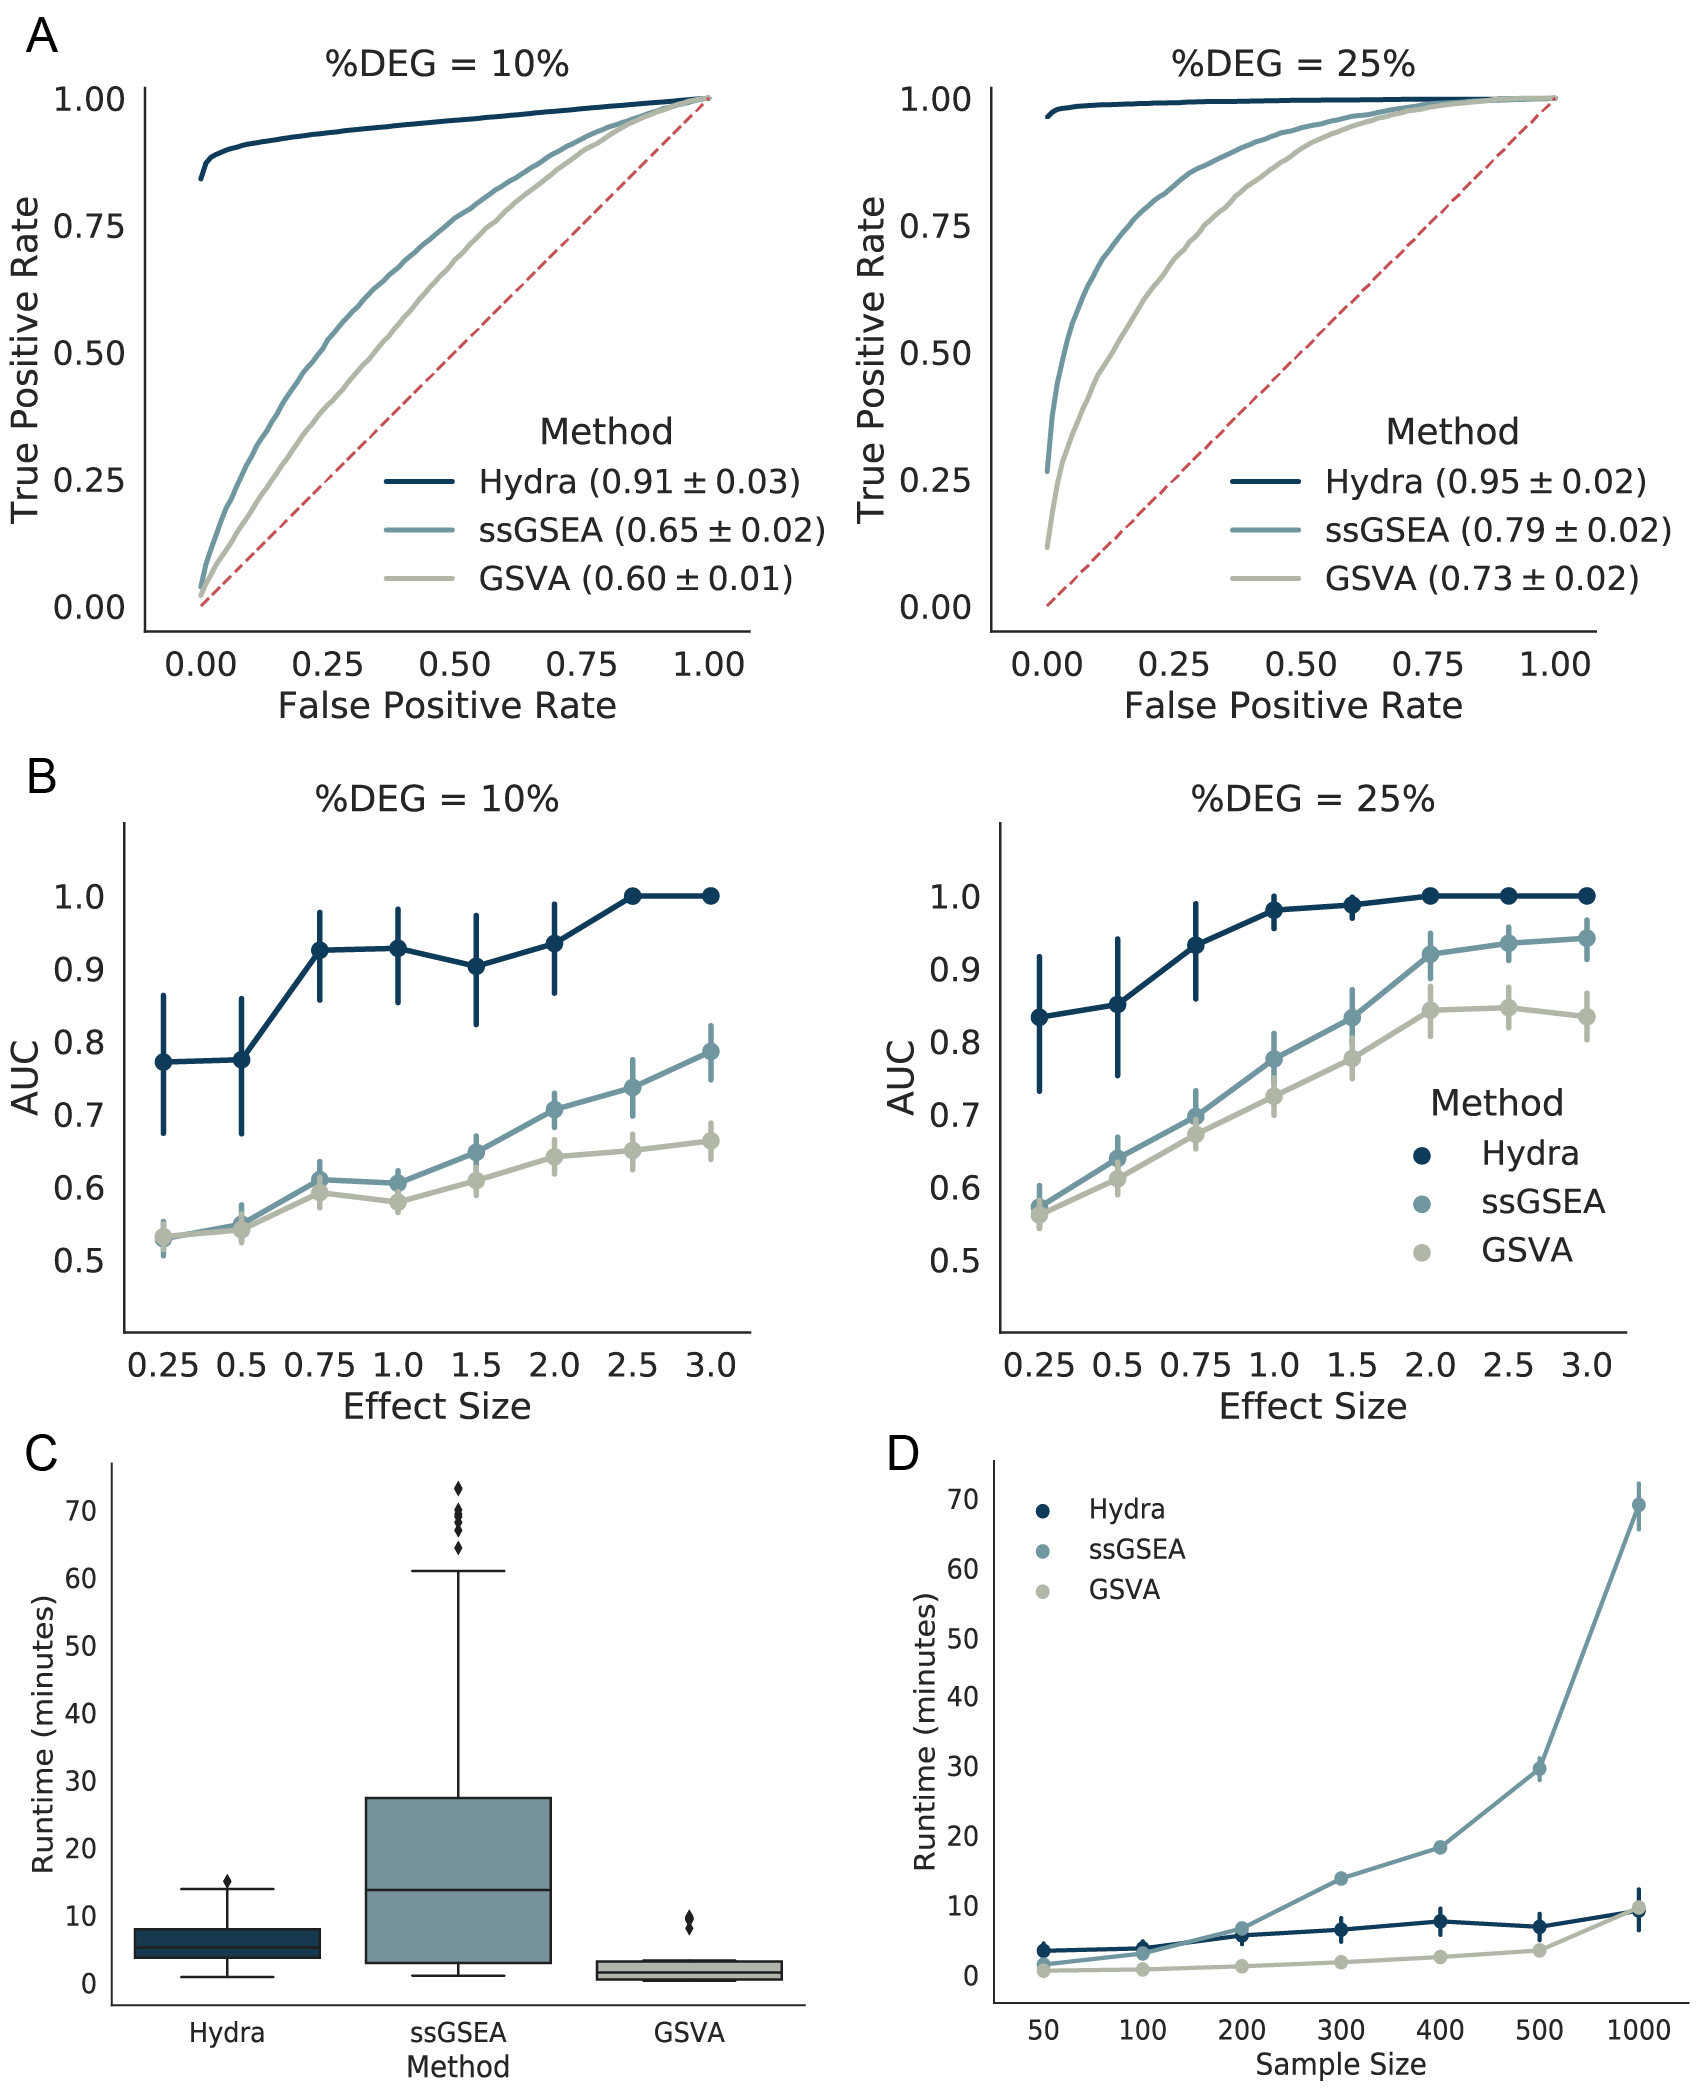
\includegraphics[width=\textwidth]{img/PNG/ROC-PLOT-V2-2x}
	\caption{{\bf Hydra \textit{sweep} is more sensitive than existing gene set enrichment approaches for detecting differential pathway expression in synthetic data and scales well to large datasets.}
		A: Mean receiver operator curves across effect sizes, percent differentially expressed genes (\%DEG), and MSigDB Hallmark gene sets. A larger area under the curve (AUC) indicates better performance. The average AUC and 95\% confidence interval for each method are in the ROC plot figure legends. B: Line plots comparing the mean AUC across a range of effect sizes and \%DEG values. C: Box plot showing mean runtimes for differential pathway analysis where the effect size is fixed but the sample size varies. D: Line plot comparing the mean runtimes for differential pathway analysis across a range of sample sizes.
		\label{rocplot}}
\end{figure}

We further investigated the performance of these methods by plotting the AUC against the effect size at 10 and 25\%DEG (Fig \ref{rocplot}B). The hydra method performed better across all effect sizes, achieving near perfect performance above an effect size of 2.0 and 0.75 at 10 and 25\%DEG, respectively. ssGSEA and GSVA performed similarly at low effect sizes, but ssGSEA performed better than GSVA as the effect size increased. Overall, the hydra framework performed significantly better than these standard gene set enrichment approaches, particularly at low effect sizes. Therefore, the hydra approach is better suited for subtyping within a disease cohort when the effect sizes are smaller and fewer genes are differentially expressed.

We performed a runtime analysis comparing hydra \textit{sweep}, ssGSEA, and GSVA for identifying a single differentially expressed gene set, since these methods are directly comparable. The average runtime for the hydra \textit{sweep} algorithm was similar to the ssGSEA to run, but the hydra runtimes were more variable across effect-sizes and number of differentially expressed genes. The GSVA approach was faster than hydra \textit{sweep} and ssGSEA, but GSVA performed worse on the synthetic data analysis than ssGSEA and hydra. We repeated the above analysis, but with an effect size of 1.0, a \%DEG of 25\%, and a range of sample sizes, including  50, 100, 200, 300, 400, 500, 1000 samples. The hydra \textit{sweep} and GSVA methods scaled well to large sample sizes, but the ssGSEA runtime increased exponentially as the sample size increased (Fig \ref{rocplot}C \& D).

\subsection*{Hydra analysis of high-risk neuroblastoma}
High-risk neuroblastoma is an aggressive disease and is resistant to intensive therapy. Further subtyping of high-risk neuroblastoma may identify novel therapeutic targets and improve risk stratification. We hypothesized that unsupervised clustering of multimodally expressed genes associated with enriched Gene Ontology terms would identify expression subtypes of high-risk neuroblastoma tumors. TumorMap  analysis \cite{newtonTumorMapExploringMolecular2017} showed that the MYCN-non-amplified (MYCN-NA) neuroblastoma samples clustered separately from MYCN-amplified (MYCN-A) and stage 4S neuroblastoma samples (\nameref{S2_Fig}). We focused on the MYCN-NA neuroblastoma tumor samples because this is the largest set of samples (N=70) and variation within MYCN-NA tumors is not well understood \cite{morgensternChallengeDefiningUltrahighrisk2019}.

We applied the hydra \textit{filter} analysis to the TARGET high-risk neuroblastoma cohort as described above. This analysis identified 931 genes within the MYCN-NA neuroblastoma cohort with a multimodal expression distribution. Of the 931 multimodally expressed genes, 358 genes were found to be potentially druggable by the Drug Gene Interaction Database (DGiDB) and 61 genes were associated with an FDA-approved, anti-neoplastic drug  \cite{cotto2017dgidb}.

We next looked to see if unsupervised clustering of multimodally expressed genes revealed coordinated expression of annotated gene sets within the MSigDB database. Applying the hydra \textit{sweep} command to the MYCN-NA neuroblastoma cohort discovered 105 gene sets with multimodal expression patterns. Each differentially expressed gene set sheds light on biological themes that are differentially expressed within the MYCN-NA neuroblastoma cohort. We clustered the differentially expressed gene sets to reveal these biological themes (\nameref{S1_Fig}). We found 6 major themes, including annotated cancer functions, cell cycle regulation, cell signaling pathways, immune functions, extracellular matrix reorganization, and metabolic pathway gene sets.

We applied the hydra \textit{enrich} analysis to the MYCN-NA cohort to identify how the most highly enriched gene sets interact to form expression subtypes. This analysis found 428 genes with a minor component probability greater than 20\% (\nameref{S1_File}). Gene Ontology analysis found enrichment for the following GO terms (FDR: q $<$ 0.01): adaptive immune response (24 genes), mesenchyme development (12 genes), steroid hormone secretion (4 genes), and response to corticosterone (4 genes). DP-GMM analysis of the 44 enriched GO term genes identified three clusters of neuroblastoma samples (Fig \ref{MYCN-NA}A). The posterior probability for belonging to each cluster was 42\%, 34\%, and 17\% for clusters 1, 2, and 3, respectively. The posterior probability for a sample belonging to a new cluster was about 6\% in our analysis.

We next investigated cluster-specific expression signatures using GSEA (see Hydra Method section). Cluster 1 was enriched for adaptive immune response gene sets, cluster 2 was enriched for proliferative signaling gene sets, and cluster 3 was enriched for cancer-associated fibroblast gene sets (Fig \ref{MYCN-NA}B). Cluster 3 shares several features of a wound healing response, including fibroblast recruitment, extracellular matrix organization, and infiltration of immune cells \cite{fosterEvolvingRelationshipWound}.

% TODO Link supplemental tables
\begin{figure}[!h]
	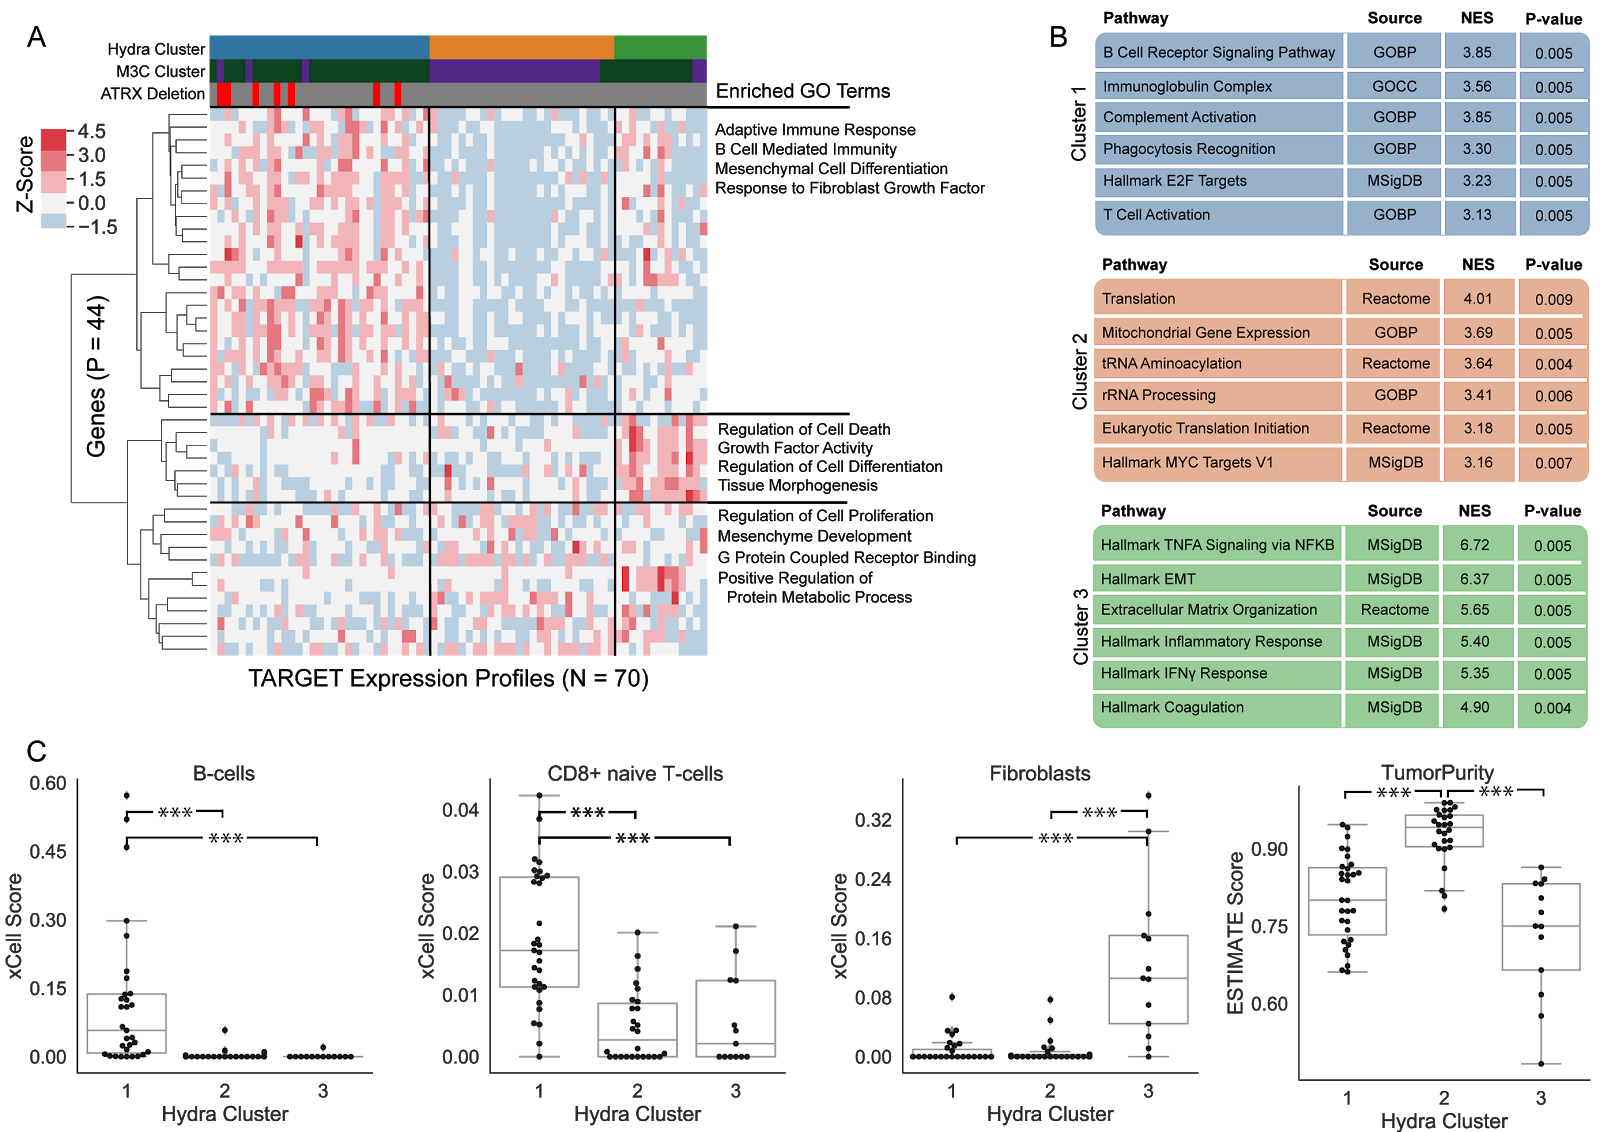
\includegraphics[width=\textwidth]{img/PNG/MYCN-NA-Figure-V5@2x}
	\caption{{\bf Hydra analysis identifies three distinct tumor microenvironment expression subtypes in MYCN non-amplified neuroblastoma samples.}
	A: Gene expression heatmap displaying expression profiles of hydra clusters. Heatmap columns (samples) are ordered by hydra cluster membership. Ward hierarchical clustering applied to rows (genes) identified coordinated expression of GO term genes. These GO term genes were originally identified by the hydra \textit{enrich} command. B: GSEA performed on each cluster identified enrichment of tumor microenvironment and proliferative signaling gene sets. C: xCell enrichment score distributions for B-cells, CD8+ naive T-cells, and Fibroblasts, and the ESTIMATE TumorPurity score distributions for each cluster; enrichments for all cell types are available in \nameref{S1_File}. Abbreviations: Normalized Enrichment Score (NES), Epithelial to Mesenchymal Transition (EMT), Gene Ontology Biological Process (GOBP).
	\label{MYCN-NA}}
\end{figure}

% See if I can compare it to another disease
Clusters 1 and 3 were enriched for tumor microenvironment-associated gene expression. To further validate this signal, we correlated the hydra clusters with enrichment scores from the tumor microenvironment profiling tools xCell \cite{aranXCellDigitallyPortraying2017} and ESTIMATE \cite{yoshiharaInferringTumourPurity2013a}. Cluster 1 had high average xCell enrichment scores associated with adaptive immune cell types including B-cells, CD4+ naive T-cells, and CD8+ naive T-cells (Kruskal-Wallis: p $<$ 0.001). Cluster 2 was characterized by the absence of immune and stromal expression and higher tumor purity scores than clusters 1 and 3. The average ESTIMATE tumor purity was 88\%, 96\% and 82\% for clusters 1, 2, and 3, respectively. Cluster 3 was enriched for fibroblast-associated expression by xCell analysis (Kruskal-Wallis: p $<$ 0.001). Clusters 1 and 3 had higher ESTIMATE immune-associated expression levels than cluster 2 (average ImmuneScore per cluster: 58, -612, 56), but cluster 3 had the highest stromal expression signature score (average StromalScore per cluster: -1027, -1310, -135). Comparing ESTIMATE enrichment scores across clusters reveals clear trends in broad immune and stromal expression signatures. Lastly, we identified a correlation between the hydra identified tumor microenvironment subtype and CD274 and CTLA4 expression (\nameref{S6_Fig})

We next correlated clusters with clinical features. We found no difference in patient survival outcomes across clusters (log-rank test, p $>$ 0.05). Notably, cluster 1, which had the highest adaptive immune expression signal in MYCN-NA neuroblastoma, over-expresses cell-cycle regulation genes, which was not observed in other small blue cell tumors. We investigated associations with clinical covariates mutation burden, age, and tumor content as assessed by a clinical pathologist, but found no statistically significant differences (Kruskal-Wallis: p $>$ 0.05). We then investigated associations between the hydra clusters and neuroblastoma-associated molecular aberrations and clinical features (Supplementary Table 6). ATRX gene deletions were enriched in cluster 1 (Fisher’s Exact Test: p $<$ 0.05). MKI low tumors were enriched in cluster 2 and 3 (Fisher’s Exact Test: p $<$ 0.01). Chromosome 17 wild-type tumors were enriched in clusters 2 and 3 (Fisher’s Exact Test: p $<$ 0.01 ). Analysis on a larger dataset may reveal additional clusters and correlations with clinical features.

Consensus clustering is a widely used approach for identifying tumor subtypes using gene expression data. We applied the M3C consensus clustering method, which is a more sophisticated version of consensus clustering that uses a null distribution to assess the statistical significance of the clustering \cite{johnM3CMonteCarlo2018, wilkersonConsensusClusterPlusClassDiscovery2010a}. We used the top 5000 genes with the largest median absolute deviation (MAD) because this threshold is routinely used in unsupervised clustering of cancer gene expression data \cite{bourgonIndependentFilteringIncreases2010, tritchlerFilteringGenesCluster2009, carcamo-oriveAnalysisTranscriptionalVariability2017}.

The M3C analysis resulted in the identification of two statistically significant clusters. One M3C cluster correlated with hydra clusters 1 and 3 and the other M3C cluster correlated with hydra cluster 2. Therefore, M3C clustering detected the tumor purity signal in the expression data, but was not able to separate the adaptive immune cell and fibroblast infiltrated clusters (hydra clusters 1 and 3). We also applied k-means clustering using the gap statistic approach \cite{tibshirani2001estimating,maechler2012cluster} for estimating the number of clusters, but this approach grouped all samples into a single cluster. We tested a range of MAD thresholds based on the median absolute deviation, but found similar results across thresholds (\nameref{S3_Fig}). Overall, the hydra approach was more sensitive at detecting distinct tumor microenvironment states than these other popular clustering methods.

To further investigate expression patterns within the hydra-identified tumor microenvironment subtypes, we performed GSEA by z-score normalizing each tumor’s gene expression data to its tumor microenvironment cluster. This is a novel GSEA approach that uses the tumor microenvironment state discovered by the hydra method to identify additional gene expression signals for individual samples. This approach revealed signals not present at the cohort level analysis (Fig \ref{subcluster}). For example, enrichment of immune expression signatures within cluster 2 predicted differences in overall survival such that patients with higher immune expression had a better overall survival rate. Similarly, an elevated cell cycle signal within cluster 3 predicted worse survival compared to other cluster 3 samples with lower cell cycle expression. A metastatic expression signal was identified in the analysis of cluster 1 samples, but this signature did not correlate with a difference in survival. This approach may therefore provide a more appropriate background distribution for revealing and evaluating the significance of gene expression patterns and survival statistics within tumor subtypes.


\begin{figure}[!h]
	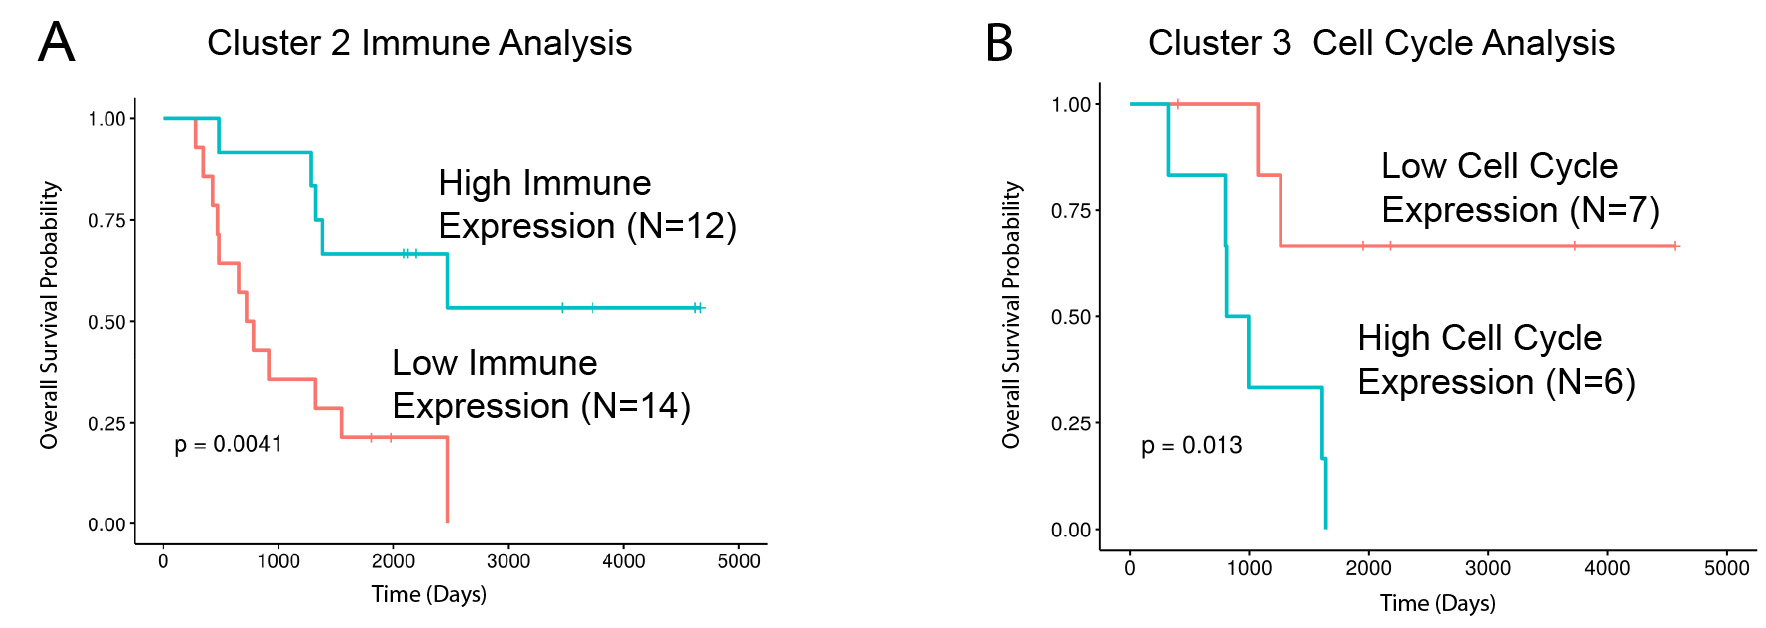
\includegraphics[width=\textwidth]{img/PNG/SubCluster-Survival-V1-2x}
	\caption{{\bf Gene set enrichment analysis (GSEA) of MYCN-NA neuroblastoma identifies survival differences within hydra cluster 2 and cluster 3.}
		Top 5 differentially enriched gene sets for each cluster comparing the entire MYCN-NA neuroblastoma cohort (cohort-level GSEA) and the corresponding hydra cluster (cluster-level GSEA). GSEA analysis of the hydra clusters found immune and cell cycle signals that were not identified in the cohort-level analysis. B: cluster-level GSEA separated cluster 2 into high and low immune subtypes. C: cluster-level GSEA separated cluster 3 into high and low cell cycle subtypes.}
	\label{subcluster}
\end{figure}

\subsection*{N-of-1 tumor analysis for pediatric neuroblastoma}
We investigated the predictive performance of the hydra approach for identifying clinically relevant signals in the N-of-1 tumor analysis setting. The command-line interface of the hydra toolkit includes a \textit{predict} function for labeling samples using a pre-fit model. The MYCN-NA neuroblastoma model described above was used to predict expression subtypes on a new set of samples. We obtained tumor gene expression data from six stage 4, MYCN-NA neuroblastoma samples from the UCSC Treehouse gene expression compendium \cite{newtonTumorMapExploringMolecular2017, vaskeComparativeTumorRNA2019}. The age at diagnosis ranged from 2 to 6 years. Four out of six samples had a deletion in the ATRX gene. Samples 1D and 1R were diagnosis and resection samples from the same patient. Most of the samples (4 out of 6) clustered in cluster 1, which is characterized by adaptive immune pathway expression. H\&E image analysis confirmed the presence of moderate levels of inflammation in 3 cluster 1 samples, minimal inflammation in the cluster 2 sample, and moderate levels of inflammation and necrosis in the cluster 3 sample (\nameref{S5_Fig}).

Three of the ATRX-deleted samples clustered with the high immune expression cluster (cluster 1) and one clustered in the low immune, high proliferative signaling cluster (cluster 2). Hydra analysis assigned sample 1D to cluster 1 and sample 1R to cluster 2 despite both samples originating from the same patient. The resection sample 1R was extracted from lymph node tissue, which has a significantly different cellular composition than the training data. Another possible explanation for the different cluster assignments is that the tumor microenvironment is dynamic and the tumor may evade immune recognition as the disease progresses, resulting in different expression signatures. We performed GSEA comparing samples 1D and 1R to investigate potential mechanisms leading to immune evasion in sample 1R. GSEA found downregulation of the MHC Class I Antigen Processing \& Presentation GO term in sample 1R (adjusted p-value $<$ 0.002). Loss of antigen processing functions is a common mechanism of immune evasion across cancer types \cite{reevesAntigenProcessingImmune2017}. We showed earlier that tumors with ATRX deletions tend to have higher immune expression, so our N-of-1 analysis on a new set of MYCN-NA neuroblastoma is consistent with our earlier analysis.


\subsection*{Hydra analysis discovers complex tissue signatures}
While the MYCN-NA neuroblastoma analysis above focused on immune and wound healing expression signatures, the hydra \textit{enrich} method is unsupervised and can therefore detect any type of expression signature. To illustrate this, we applied the hydra \textit{filter}/\textit{enrich} analysis to the TARGET osteosarcoma cohort (N=74) and discovered enrichment of the GO striated muscle contraction term (FDR $<$ 0.01, Fig \ref{muscle}). Multivariate clustering for the GO striated muscle contraction gene set using the \textit{sweep} routine identified two clusters. xCell analysis of the osteosarcoma cohort found significant enrichment of skeletal muscle expression in the second cluster (Mann-Whitney U test, p $<$ 0.001). Surprisingly, the M3C clustering approach was not able to detect the strong muscle signature using the 5000 genes with the largest MAD (p $>$ 0.05). We used the muscle expression signature to identify osteosarcoma tumors in the UCSC Treehouse Compendium which also contained a similar expression signature. We subsequently confirmed with a licensed pathologist that one of the muscle-expression positive tumor samples did contain significant muscle tissue infiltration. The hydra \textit{enrich} analysis is unsupervised and revealed expression signatures not routinely investigated when analyzing osteosarcoma data. Nevertheless, these signals contribute significantly to the tumor expression profile, so explaining these sources of variation is necessary to derive clinically relevant conclusions from gene expression data.

%
% Osteo Muscle Figure
%
\begin{figure}[!h]
	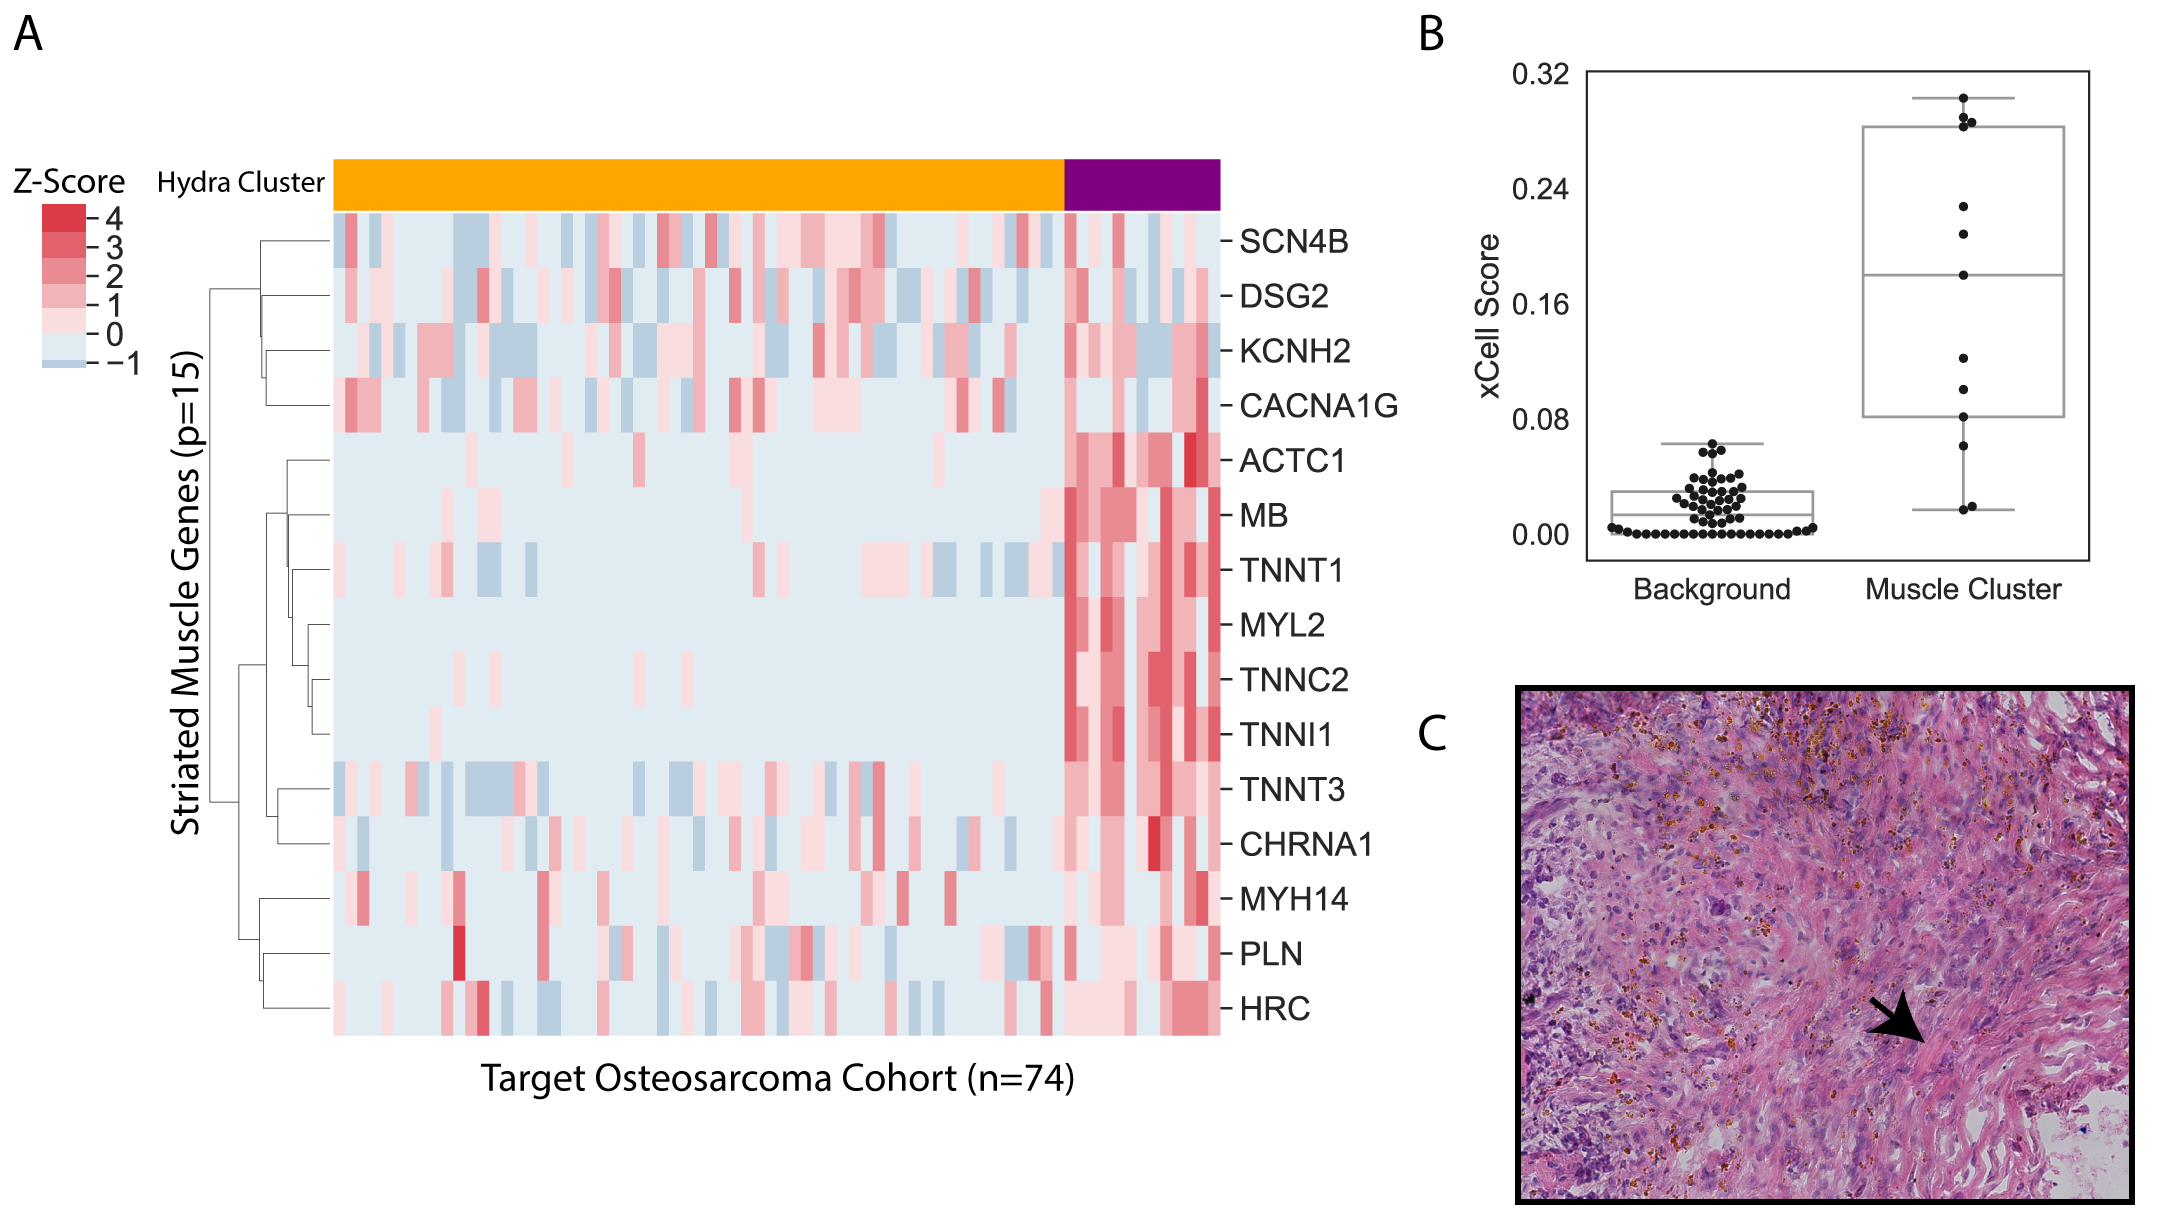
\includegraphics[width=\textwidth]{img/PNG/muscle-signature-genes-2x}
	\caption{{\bf Hydra analysis of TARGET osteosarcoma cohort reveals skeletal muscle signature.}
		 Hydra enrichment analysis on the TARGET osteosarcoma cohort revealed a subset of patients with high skeletal muscle expression. A: Clustered heatmap shows the muscle signature genes identified by hydra unsupervised enrichment analysis. B: xCell tumor microenvironment profiling identified significant differences in skeletal muscle expression compared to background (p $<$ 0.001). C: H\&E stained tumor slide for an out-of-sample osteosarcoma expression profile confirms presence of striated muscle tissue within the tumor sample.}
	\label{muscle}
\end{figure}

We applied the \textit{filter} method to Ewing sarcoma and discovered multimodal expression of an important druggable gene, JAK1. Applying the multimodal expression model allowed us to deconstruct the Ewing sarcoma distribution into three components (\nameref{S7_Fig}A). We found that the expression component with the highest JAK1 expression was also enriched for mast cell expression (\nameref{S7_Fig}B). Therefore, overexpression of JAK1 may not correspond to activation of the JAK/STAT signaling pathway in cancer cells but rather to the presence of mast cells within the tumor microenvironment. Furthermore, targeted inhibition of JAK1 using ruxolitinib was shown to inhibit essential mast cell functions, including degranulation \cite{hermansJAK1JAK2Inhibitor2018}. Therefore, therapeutic intervention intending to inhibit JAK1 expression in cancer cells may inadvertently inhibit the patient’s mast cell functions. overexpression analysis using the Ewing sarcoma JAK1 expression distribution may identify JAK1 as an actionable lead, but further investigation into the effect of inhibiting off-target JAK1 expression in mast cells is needed. The hydra framework facilitates the identification of important expression signatures which can be used to deconstruct complex tumor expression subtypes and identify potentially confounding expression signals.

We next quantified the number of multimodal druggable genes from the MYCN-NA neuroblastoma dataset that correlated with at least one xCell cell type signature. Out of the 358 druggable genes, we found that 77 correlated with a non-cancer cell type (Kruskal-Wallis test: Holm-Sidak adjusted p-value $<$ 0.05, \nameref{S1_File}). Some of the druggable genes were expected to correlate with non-cancer cells, including the cytokines IL6 and TGFB2, which correlated with epithelial cells and fibroblasts, respectively. Other druggable genes were surprising, like AURKA and AURKB, which correlated with higher Th2 cells. Aurora kinases play essential roles in spindle formation during mitosis and the overexpression of these genes is associated with evading spindle formation checkpoints in cancer \cite{marisInitialTestingAurora2010}, but little is known in how these genes correlate with infiltrating immune cells. Aurora kinase inhibitors show limited clinical activity in solid tumors, but have been shown to have a greater effect in leukemias \cite{marisInitialTestingAurora2010,gautschiAuroraKinasesAnticancer2008}.

\subsection*{Hydra analysis reveals recurrent expression subtypes across small blue round cell tumors}
We next investigated whether similar hydra clusters could be identified across other small blue round cell tumors. We first performed TumorMap analysis, which is a dimensionality reduction approach for visualizing genomic data on a 2D surface \cite{newtonTumorMapExploringMolecular2017}. We found that small blue round cell tumor types --- MYCN-NA neuroblastoma, osteosarcoma, Ewing sarcoma, synovial sarcoma, alveolar rhabdomyosarcoma, and embryonal rhabdomyosarcoma --- all form separate TumorMap clusters (Fig \ref{pancan}A). This suggests there is a strong cell-of-origin signal driving the clustering of these cancer types, which is an observation that was recently made in the larger TCGA dataset of adult cancers \cite{hoadleyCellofOriginPatternsDominate2018}. While pan-cancer analysis emphasized the differences across small blue round cell tumors, we hypothesized that expression subtypes within cancer types would participate in shared biological themes.

\begin{figure}[!h]
	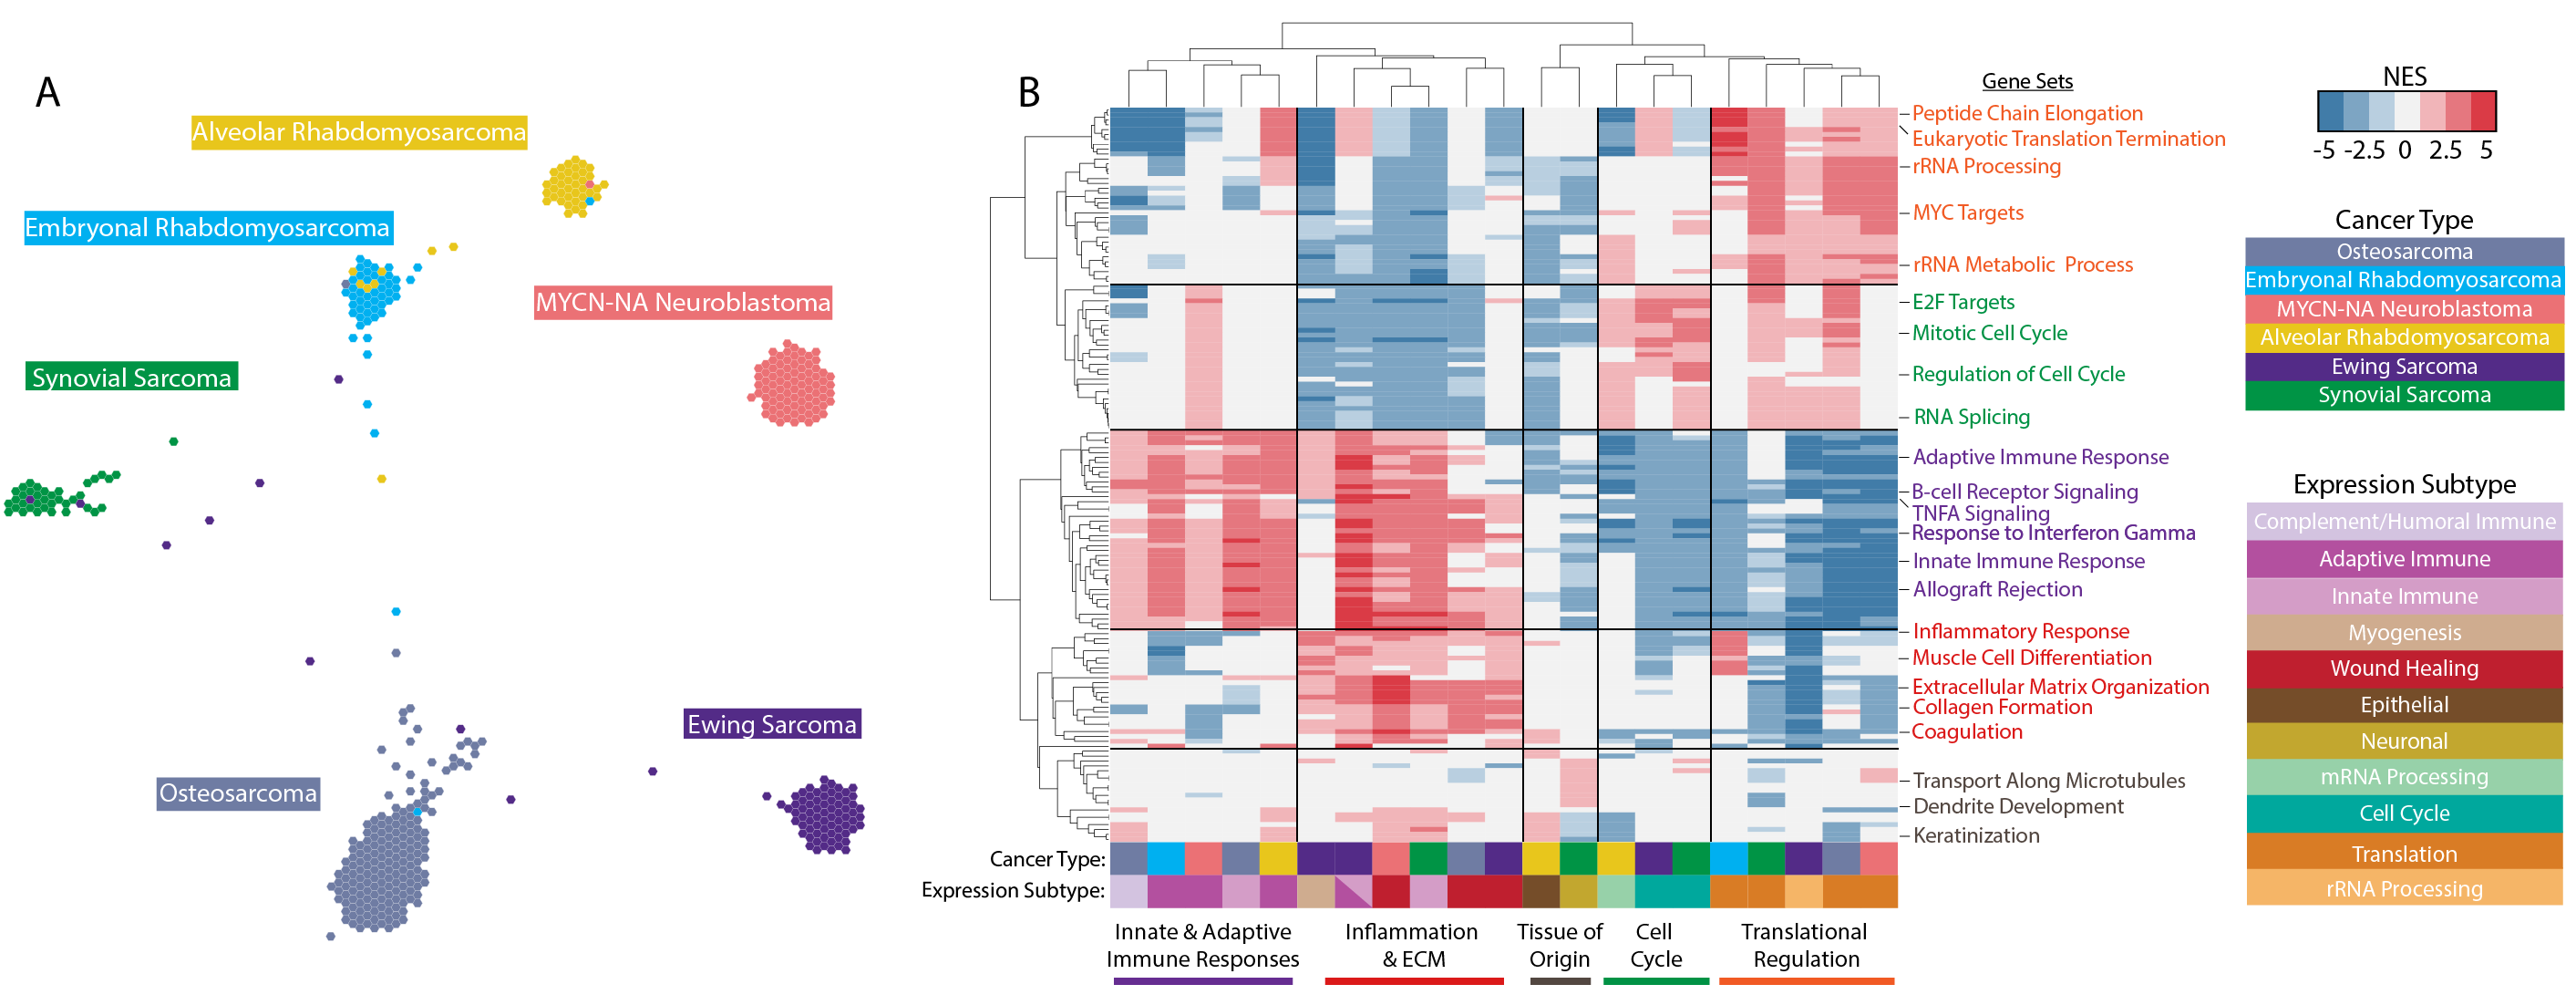
\includegraphics[width=\textwidth]{img/PNG/hydra-pan-small-round-blue-V2-2x}
	\caption{{\bf Hydra \textit{enrich} analysis of small blue round cell tumors reveals similar expression subtypes across cancer types.} A: TumorMap visualization of 6 small blue round cell tumor types. B: Hierarchically clustered heatmap for the top 10 enriched gene sets across the 21 small blue round cell tumor expression subtypes. Each column corresponds to a cancer type and an expression subtype (x-axis). Each row corresponds to a gene set. The expression subtype was manually assigned after reviewing the most highly enriched gene sets for each cancer expression subtype.}
	\label{pancan}
\end{figure}

We next performed hydra \textit{enrich} analysis within each small round blue cell cancer type and were surprised to find shared biological themes across all six small blue round tumor types. Hierarchical clustering of the top 10 statistically significant gene sets for each cancer type resulted in clustering by expression subtype and not the cancer type (Fig \ref{pancan}B). Common themes emerged across diseases including translational regulation, cell cycle regulation, immune effector cell signaling, inflammation, extracellular matrix organization, and tissue-of-origin signals. Furthermore, these signals predicted differences in patient outcomes in osteosarcoma and synovial sarcoma (Fig \ref{surv}). In both cases, the presence of immune associated expression correlated with better patient outcomes compared to tumors with proliferative signaling pathways associated with the upregulation of translation initiation. Other osteosarcoma clusters were not included in the survival analysis due to insufficient number of samples with survival data. Survival data were not available for the rhabdomyosarcoma and Ewing sarcoma expression datasets.

%
% Osteo-Synovial Survival
%

\begin{figure}[!h]
	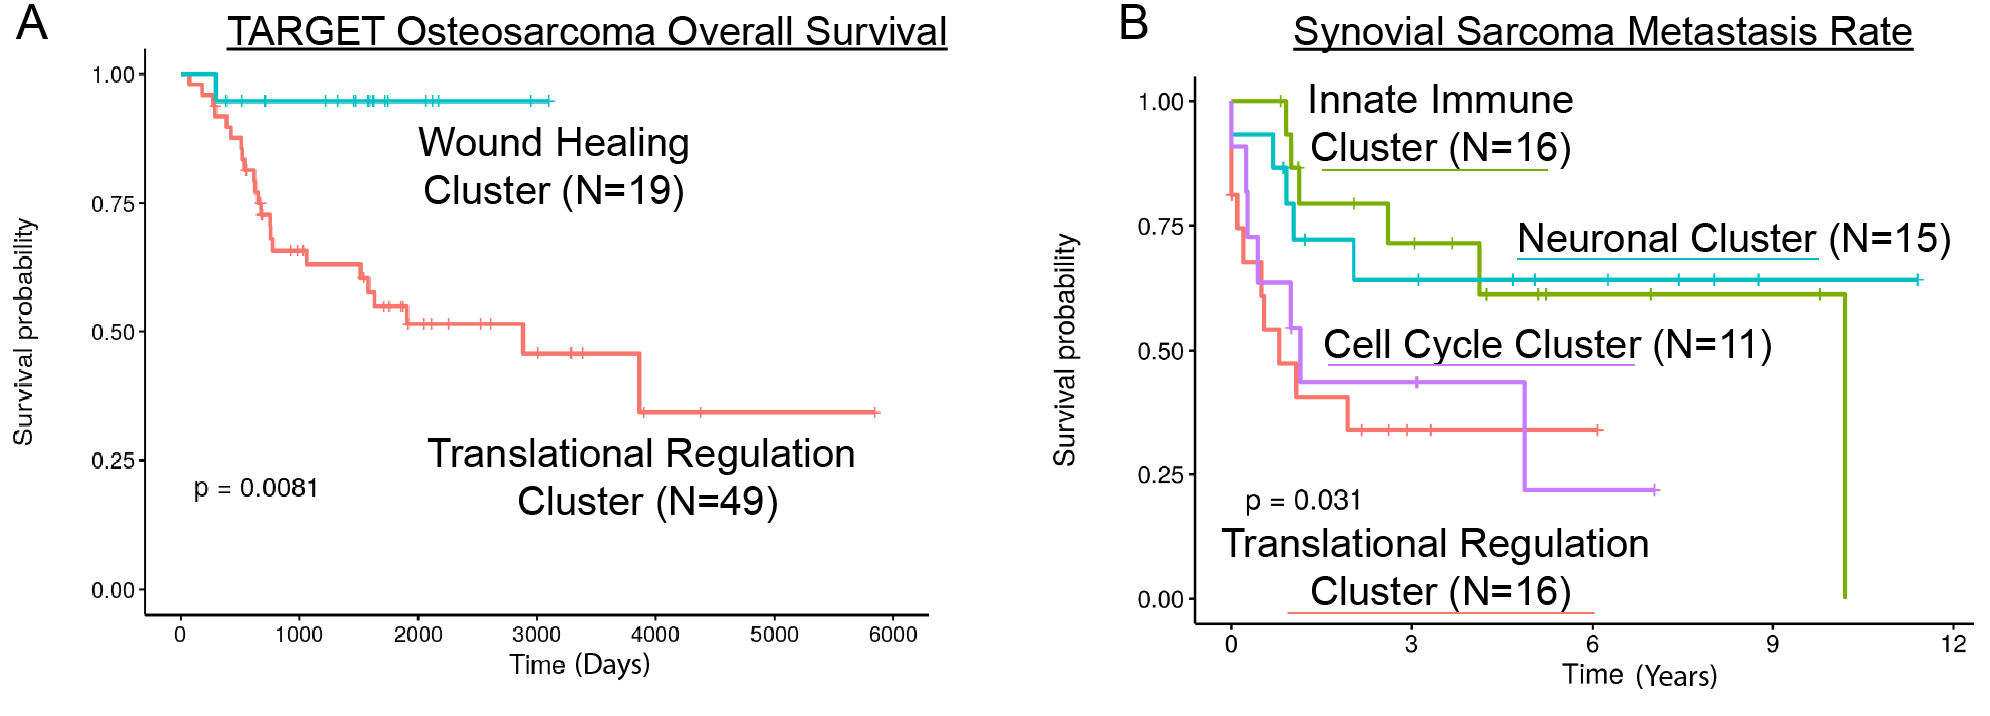
\includegraphics[width=\textwidth]{img/PNG/osteosarcoma-synovial-survival-2x}
	\caption{{\bf Hydra analysis identifies tumor microenvironment expression subtypes that correlate with patient outcomes in osteosarcoma and synovial sarcoma.} A: Kaplan-Meier plot showing overall survival curves for osteosarcoma wound healing and translation clusters. B: Kaplan-Meier plot showing metastasis survival curves for synovial sarcoma clusters.}
	\label{surv}
\end{figure}

\section*{Discussion}
The hydra framework uses model-based clustering to facilitate the discovery of recurrent expression patterns within cancer gene expression cohorts. We leveraged recent improvements in model-based clustering algorithms to identify differentially expressed genes without a matched normal distribution. We modeled differential expression as a multimodal Gaussian distribution using nonparametric Bayesian statistics. We then enriched for biologically-annotated Gene Ontology terms and performed multivariate clustering to reveal expression subtypes. The hydra framework can be used for both identifying expression subtypes within large cohorts and classifying new tumor gene expression profiles using the trained models. The hydra framework outperformed standard gene set enrichment tools for identifying overexpression of the MSigDB Hallmark cancer gene sets in synthetic data. Application of this framework to small blue round cell tumors identified shared biological themes associated with the tumor microenvironment.

Multivariate gene expression analysis is typically underpowered because the number of genes greatly exceeds the number of samples. To address this limitation, we propose selecting for multimodally expressed genes before performing multivariate analysis. The hydra \textit{filter} reduces the number of genes and enriches for genes that participate in known biological processes, including those curated in the Gene Ontology and MSigDB databases. Furthermore, we found that multimodally expressed genes improves separation of known clinical subtypes better by TumorMap analysis compared to the standard approach of using all expressed genes (\nameref{S2_Fig}). Furthermore, we showed that the hydra approach is more sensitive at identifying differential pathway expression and resolving tumor microenvironment subtypes than single-sample GSEA methods and consensus clustering approaches, respectively.

Significant progress has been made in subtyping neuroblastomas and adapting therapy for aggressive subtypes, but unexplained heterogeneity remains \cite{morgensternChallengeDefiningUltrahighrisk2019}. Failure to account for this heterogeneity decreases the power of standard methods to detect important expression patterns. Identifying biomarkers using genome-wide technology may lead to improved risk stratification and the discovery of novel drug targets. Hydra analysis of the TARGET MYCN-NA neuroblastoma cohort found differential expression of tumor microenvironment markers, including markers of the adaptive immune response. Pediatric cancers are generally thought to be less immunogenic because they have lower mutation burdens than adult cancers, but the immunogenicity of pediatric cancer has not been sufficiently investigated \cite{majzner2017harnessing, zamoraPediatricPatientsAcute2019}.

Our analysis found significant variation in immune marker expression, including markers of response to checkpoint blockade therapy, and identified ATRX deletions as a potential biomarker of immune infiltrated tumors in MYCN-NA neuroblastoma. Analysis of other small blue round cell tumors revealed similar expression signatures across tumor types, despite samples clustering by their histology in a pan-cancer TumorMap analysis. Identification of shared expression signatures across cancer types may suggest that these patients would respond similarly to therapies that target these pathways. In particular, the identification of a cross-disease subtype associated with high expression of immune markers may warrant further investigation of immunotherapies in small blue round cell tumors using a basket clinical trial design \cite{cunananEfficientBasketTrial2017}.

We found significant differences in immune and stromal expression that may inform precision medicine applications. The tumor microenvironment has become an important therapeutic consideration, but few methods account for the tumor microenvironment directly. Tumor purity has been identified as a confounding factor in cancer gene expression subtyping efforts \cite{rheeImpactTumorPurity2018}. For example, tumor purity and tumor microenvironment expression have been shown to correlate with pancreatic cancer subtypes \cite{raphael2017integrated}. Furthermore, Aran et al. (2018) found that tumor purity was correlated with the mesenchymal glioblastoma subtype and recommended a differential expression approach to computationally remove the tumor purity signal. However, standard approaches for subtracting the tumor purity effect may not be the best approach because several mechanisms may influence tumor purity, and each mechanism may result in a different expression pattern. For instance, our analysis of MYCN-NA neuroblastoma identified two gene expression signatures that correlated with lower predicted tumor purity. Cluster 1 had an adaptive immune expression signature and cluster 3 had a cancer-associated fibroblast signature. Therefore, we suggest that the estimated tumor purity signal should not be subtracted without first accounting for the different mechanisms influencing tumor purity.

We also found shared biological pathway enrichment across small blue round cell tumors. While these diseases are related and may derive from similar cell lineages, current expression methods often emphasize difference across these diseases (Fig \ref{pancan}A). Unsupervised clustering of adult cancer types found that cell-of-origin signals strongly influence clustering of cancer gene expression data \cite{hoadleyCellofOriginPatternsDominate2018}. Although these diseases have distinct expression patterns on the surface, we discovered common themes once we subset the data to the cell-of-origin signal and applied the hydra analysis tools. 

There appear to be at least three major tumor microenvironment states: immune silent, immune infiltrated, and wound healing subtypes. The immune infiltrated and wound healing subtypes predicted better overall survival in osteosarcoma and delayed metastases in synovial sarcoma tumors, which suggests the involvement of the host immune response limits the progression of these tumors. Amplification of the host immune response may further limit tumor growth and lead to immune-mediated tumor cell death. Additional research into the immune modulating therapies is warranted in small blue round cell tumors and may lead to improved outcomes for some patients.

\section*{Conclusion}
Precision oncology aims to differentiate tumors of the same diagnosis in order to match patients with the best treatment. We have developed the hydra framework to discover subtle but recurrent expression patterns within a cohort of samples with the same diagnosis, which is a novel strategy for pediatric precision oncology research. Our approach may help to uncover the biology underlying tumor progression and response to therapy. We have shown that hydra is more sensitive than standard gene set enrichment approaches for detecting differential pathway expression. Additionally, our framework provides tools to conduct unsupervised clustering analysis to discover expression subtypes. We applied the unsupervised hydra analysis to small blue round cell tumors and discovered distinct tumor microenvironment states. This shows that one of the strongest signals in clinical gene expression data comes from the TME, so careful modeling of the TME is required to maximize the impact of clinical gene expression analysis. The hydra framework provides unbiased clustering tools to characterize these sources of variation in specific disease populations and identify shared biological themes that can potentially be targeted therapeutically.

\section*{Supporting information}

% Include only the SI item label in the paragraph heading. Use the \nameref{label} command to cite SI items in the text.
\paragraph*{S1 Fig.}
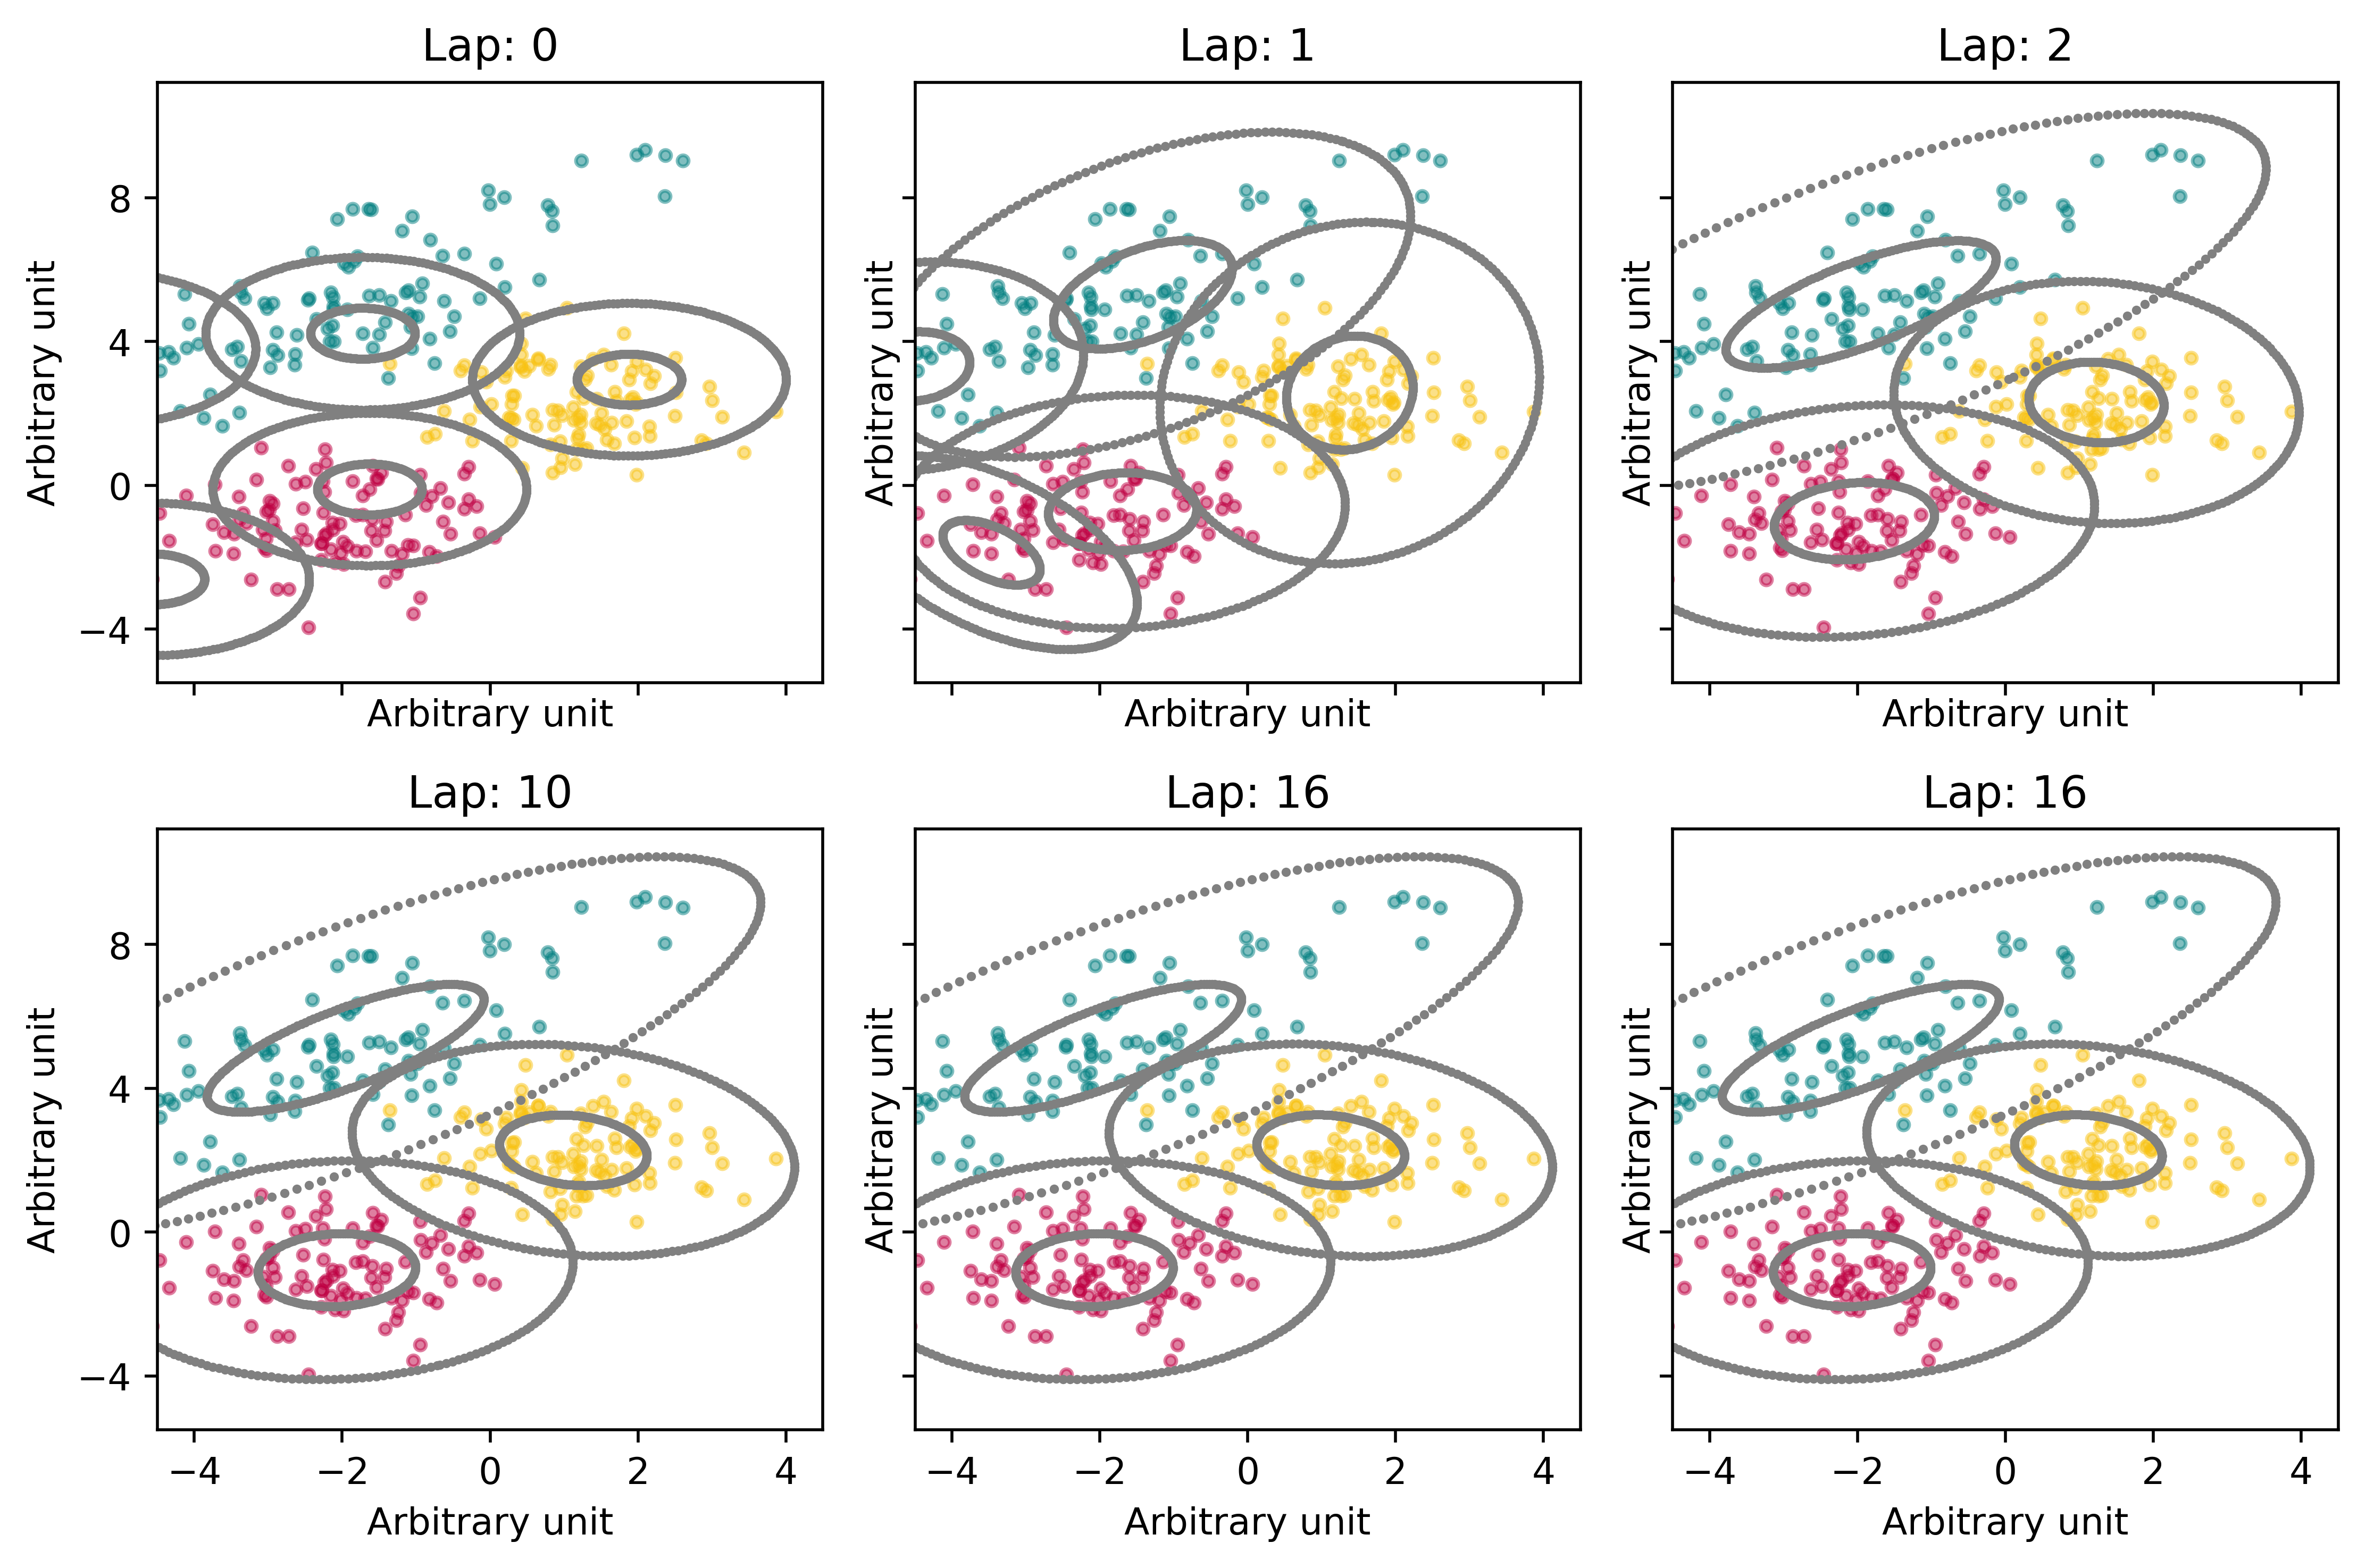
\includegraphics[width=\textwidth]{img/PNG/cluster-over-time}
\label{S1_Fig}
{\bf Example of bnpy memoized online variational inference clustering on toy data.} We used the bnpy moVB algorithm to infer the number of clusters from synthetic data. The model first randomly assigns clusters. Then, the model iteratively improves the model fit, creating and destroying clusters until the model converges on the correct number of clusters \cite{hughesBnpyReliableScalable}.

\paragraph*{S2 Fig.}
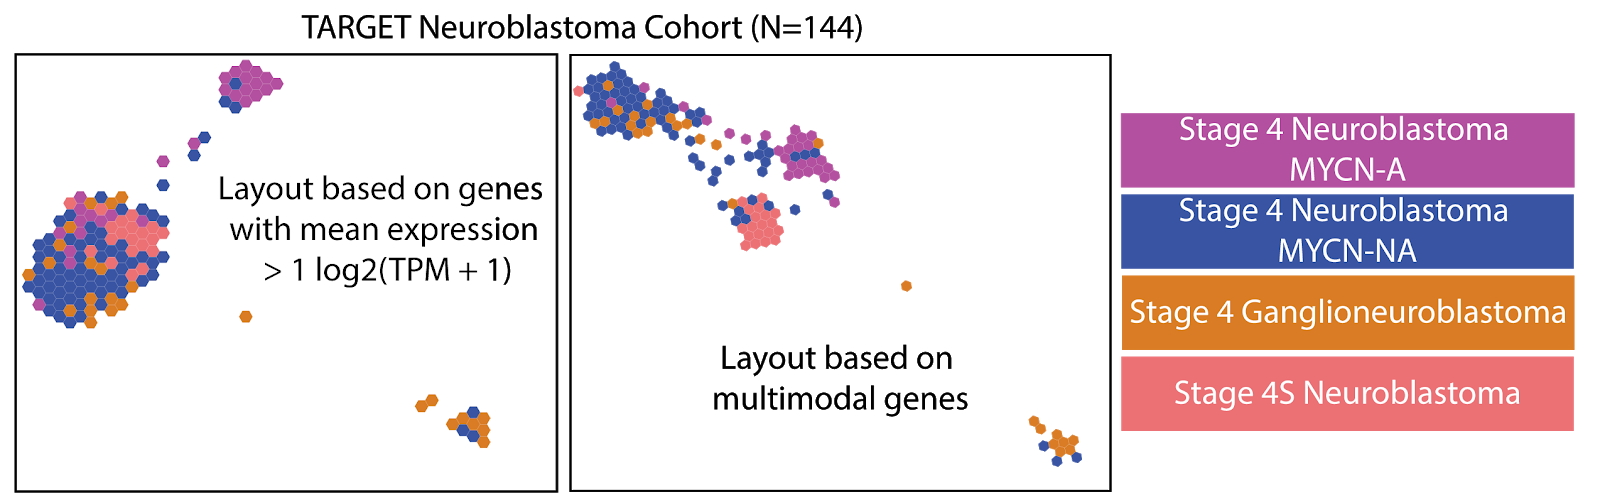
\includegraphics[width=\textwidth]{img/PNG/TumorMap-NBL-MM-V3-2x}
\label{S2_Fig}
{\bf Enriching for multimodally expressed genes improves clustering of established neuroblastoma subtypes.} Standard TumorMap analysis (Newton et al. 2017) of the TARGET neuroblastoma dataset resulted in stage 4S samples clustering with stage 4 neuroblastoma samples (left). An alternative TumorMap based solely on 1,498 multimodally expressed genes separated the stage 4S samples into a distinct cluster (right).

\paragraph*{S3 Fig.}
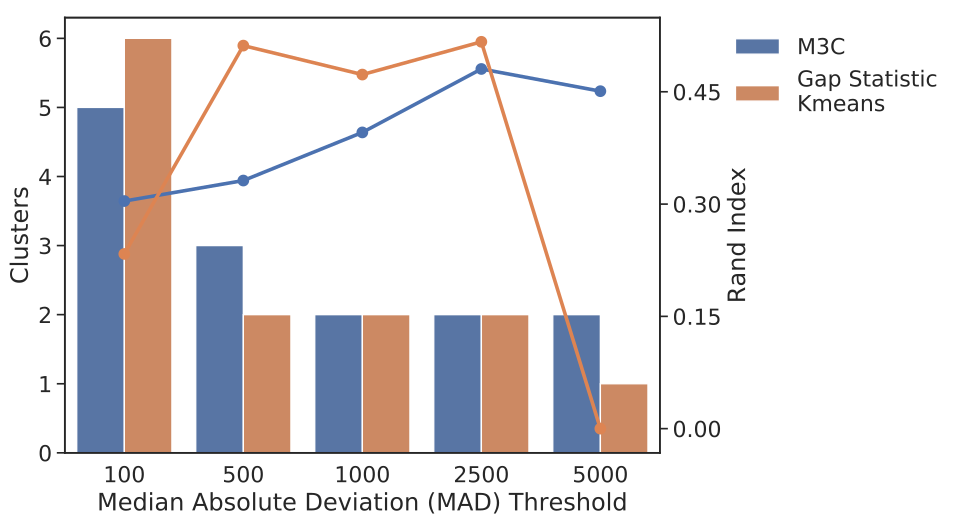
\includegraphics[width=0.75\textwidth]{img/PNG/clustering-screen}
\label{S3_Fig}
{\bf{Consensus and k-means clustering applied to TARGET MYCN-NA dataset.}} We tested a range of gene expression variation thresholds based on the median absolute deviation, but found that the clusters identified by this approach could not resolve the same clusters as the hydra approach. The barplot shows the number of clusters and the lineplot tracks the Rand index comparing the M3C and k-means clusters and the hydra clusters.

\paragraph*{S4 Fig.}
\includegraphics[width=\textwidth]{img/PNG/sweep-gene set-network-V4-2x}
\label{S4_Fig}{\bf Hydra \textit{sweep} analysis reveals differential pathway expression with MYCN-NA neuroblastoma without a matched cohort of normal tissue.}
Unsupervised clustering of multimodal gene sets revealed biological themes associated with cancer functions. cell cycle, immune functions, extracellular matrix organization, and metabolism.

\paragraph*{S5 Fig.}
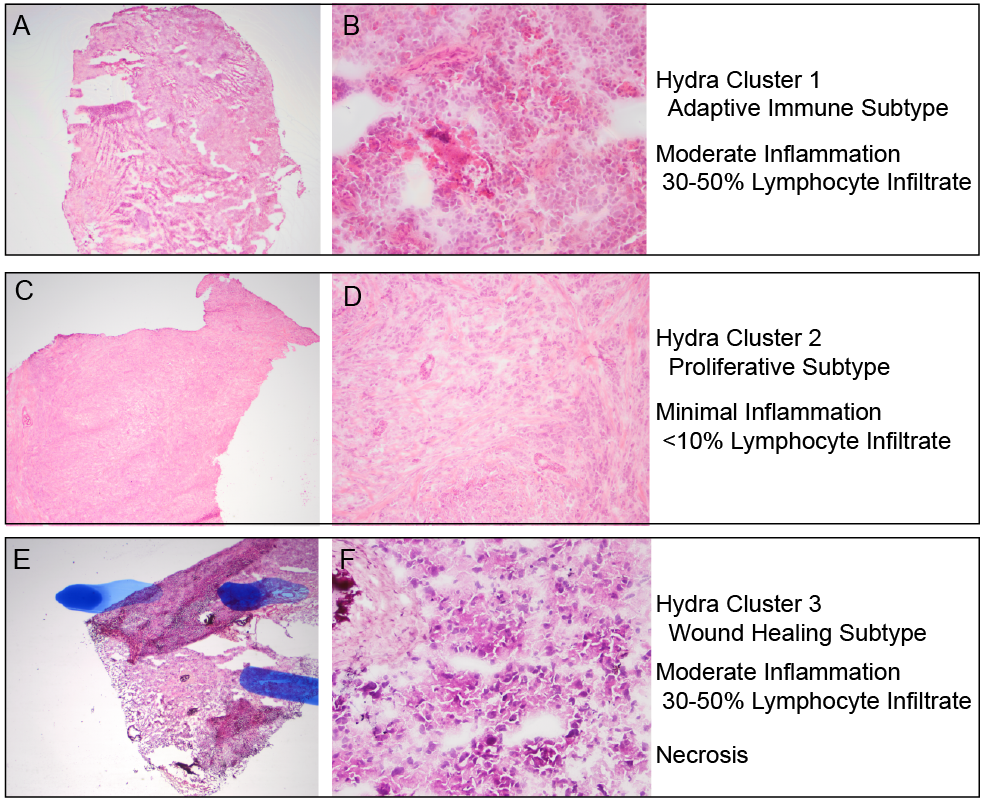
\includegraphics[width=\textwidth]{img/PNG/HE-Figure-3-Clusters-2x}
\label{S5_Fig} {\bf Hydra method correlates with distinct tumor features as assessed by licensed pathologist review of tumor H\&E slides.}
A-B: H\&E sections from fresh frozen tumor tissue from MYCN-NA neuroblastoma sample at A: 2X magnification and B: 20X magnification. Tumor cells are medium to large with moderate amounts of cytoplasm and areas of rhabdoid appearing undifferentiated cells.  There is a moderate amount of mixed inflammation present (30-50\%) consisting mostly of mature mononuclear cells with some plasma cells and scattered eosinophils. C-D: H\&E sections from fresh frozen tumor tissue from MYCN-NA neuroblastoma at C: 2X magnification and D: 20X magnification. Tumor cells are moderate to large in size with moderate amounts of cytoplasm. There is a minimal amount ($<$10\%) of apparent mononuclear inflammation scattered throughout the tumor. E-F: H\&E sections from fresh frozen tumor tissue from MYCN-NA neuroblastoma sample at (E) 2X magnification and (F) 20X magnification.  Tumor cells are medium to large with moderate amounts of cytoplasm and areas of rhabdoid appearing undifferentiated cells.  There are also areas of apparent necrosis.  There is a moderate amount of inflammation present (30-50\%) consisting mostly of mature mononuclear cells with some plasma cells and scattered eosinophils.

% Add panel labels
\paragraph*{S6 Fig.}
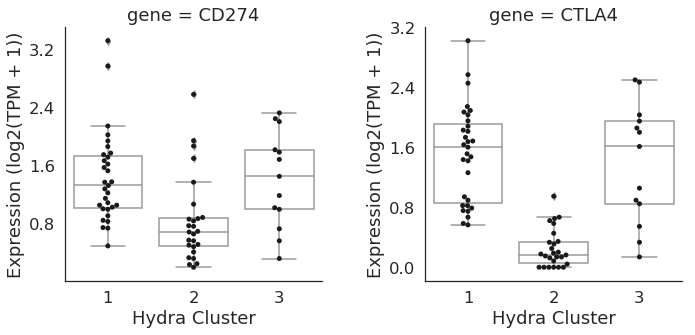
\includegraphics[width=\textwidth]{img/PNG/Checkpoint-Plots-V1}
\label{S6_Fig} {\bf Hydra \textit{enrich} analysis identifies correlation between expression subtypes and checkpoint blockade markers in MYCN-NA neuroblastoma.}

% Add panel labels
\paragraph*{S7 Fig.}
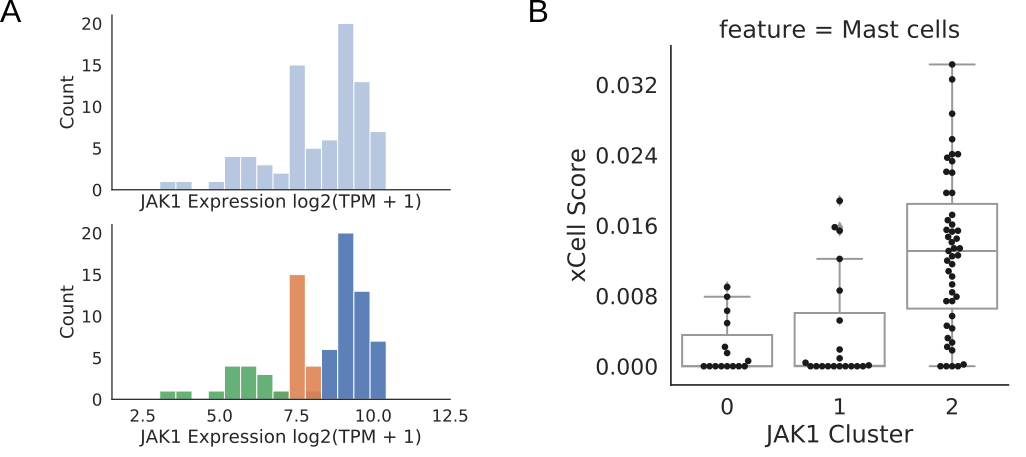
\includegraphics[width=\textwidth]{img/PNG/ewing-jak1-expression-fig}
\label{S7_Fig} {\bf Hydra analysis identifies correlation between expression of druggable JAK1 gene and mast cell expression signature in Ewing sarcoma.} A: We show the utility of the mixture model approach for identifying important gene expression patterns for precision medicine applications. JAK1 is a druggable gene, but JAK1 is also an important gene in immune cell signaling pathways. B: Boxplot showing the xCell mast cell enrichment score for three clusters associated with JAK1 expression.

\paragraph*{S1 File.}
\label{S1_File}
{\bf TARGET MYCN-NA neuroblastoma supplementary data.}

\paragraph*{S2 File.}
\label{S2_File}
{\bf Hydra method documentation.}

%\paragraph*{S1 Video.}
%\label{S1_Video}
%{\bf Lorem ipsum.}  Maecenas convallis mauris sit amet sem ultrices gravida. Etiam eget sapien nibh. Sed ac ipsum eget enim egestas ullamcorper nec euismod ligula. Curabitur fringilla pulvinar lectus consectetur pellentesque.

%\paragraph*{S1 Appendix.}
%\label{S1_Appendix}
%{\bf Lorem ipsum.} Maecenas convallis mauris sit amet sem ultrices gravida. Etiam eget sapien nibh. Sed ac ipsum eget enim egestas ullamcorper nec euismod ligula. Curabitur fringilla pulvinar lectus consectetur pellentesque.

%\paragraph*{S1 Table.}
%\label{S1_Table}
%{\bf Lorem ipsum.} Maecenas convallis mauris sit amet sem ultrices gravida. Etiam eget sapien nibh. Sed ac ipsum eget enim egestas ullamcorper nec euismod ligula. Curabitur fringilla pulvinar lectus consectetur pellentesque.

\section*{Acknowledgments}
We would like to thank the patients and families who participated in translational genomics research. We would also like to thank St. Baldrick's Foundation, California Precision Medicine Initiative, National Human Genome Research Institute of the National Institutes of Health for funding support.

\nolinenumbers

% Either type in your references using
% \begin{thebibliography}{}
% \bibitem{}
% Text
% \end{thebibliography}
%
% or
%
% Compile your BiBTeX database using our plos2015.bst
% style file and paste the contents of your .bbl file
% here. See http://journals.plos.org/plosone/s/latex for
% step-by-step instructions.
%

%\bibliographystyle{plos2015.bst}
%\bibliography{zotero-library}

%\begin{thebibliography}{10}
% Copy and paste bbl
%\end{thebibliography}

% TODO: REDO BIBLIOGRAPHY
\begin{thebibliography}{10}

	\bibitem{vivianToilEnablesReproducible2017}
	Vivian J, Rao AA, Nothaft FA, Ketchum C, Armstrong J, Novak A, et~al.
	\newblock Toil Enables Reproducible, Open Source, Big Biomedical Data
	Analyses;35(4):314--316.
	\newblock doi:{10.1038/nbt.3772}.

	\bibitem{pughGeneticLandscapeHighrisk2013}
	Pugh TJ, Morozova O, Attiyeh EF, Asgharzadeh S, Wei JS, Auclair D, et~al.
	\newblock The Genetic Landscape of High-Risk Neuroblastoma;45(3):279--284.
	\newblock doi:{10.1038/ng.2529}.

	\bibitem{goldmanUCSCXenaPlatform2018}
	Goldman M, Craft B, Kamath A, Brooks A, Zhu J, Haussler D.
	\newblock The {{UCSC Xena Platform}} for Cancer Genomics Data Visualization and
	Interpretation; p. 326470.
	\newblock doi:{10.1101/326470}.

	\bibitem{thecancergenomeatlasresearchnetworkCancerGenomeAtlas2013}
	{The Cancer Genome Atlas Research Network}, Weinstein JN, Collisson EA, Mills
	GB, Shaw KRM, Ozenberger BA, et~al.
	\newblock The {{Cancer Genome Atlas Pan}}-{{Cancer}} Analysis
	Project;45:1113--1120.
	\newblock doi:{10.1038/ng.2764}.

	\bibitem{newtonTumorMapExploringMolecular2017}
	Newton Y, Novak AM, Swatloski T, McColl DC, Chopra S, Graim K, et~al.
	\newblock {{TumorMap}}: {{Exploring}} the {{Molecular Similarities}} of
	{{Cancer Samples}} in an {{Interactive Portal}};77(21):e111--e114.
	\newblock doi:{10.1158/0008-5472.CAN-17-0580}.

	\bibitem{vaskeComparativeTumorRNA2019}
	Vaske OM, Bjork I, Salama SR, Beale H, Shah AT, Sanders L, et~al.
	\newblock Comparative {{Tumor RNA Sequencing Analysis}} for
	{{Difficult}}-to-{{Treat Pediatric}} and {{Young Adult Patients With
			Cancer}};2(10):e1913968--e1913968.
	\newblock doi:{10.1001/jamanetworkopen.2019.13968}.

	\bibitem{joyceCellExclusionImmune2015}
	Joyce JA, Fearon DT.
	\newblock T Cell Exclusion, Immune Privilege, and the Tumor
	Microenvironment;348(6230):74--80.
	\newblock doi:{10.1126/science.aaa6204}.

	\bibitem{chenElementsCancerImmunity2017}
	Chen DS, Mellman I.
	\newblock Elements of Cancer Immunity and the Cancer–Immune Set
	Point;541(7637):321--330.
	\newblock doi:{10.1038/nature21349}.

	\bibitem{mellmanCancerImmunotherapyComes2011}
	Mellman I, Coukos G, Dranoff G.
	\newblock Cancer Immunotherapy Comes of Age;480(7378):480--489.
	\newblock doi:{10.1038/nature10673}.

	\bibitem{pageImmuneModulationCancer2014}
	Page DB, Postow MA, Callahan MK, Allison JP, Wolchok JD.
	\newblock Immune Modulation in Cancer with Antibodies;65:185--202.
	\newblock doi:{10.1146/annurev-med-092012-112807}.

	\bibitem{majzner2017harnessing}
	Majzner RG, Heitzeneder S, Mackall CL.
	\newblock Harnessing the Immunotherapy Revolution for the Treatment of
	Childhood Cancers;31(4):476--485.

	\bibitem{zamoraPediatricPatientsAcute2019}
	Zamora AE, Crawford JC, Allen EK, Guo XzJ, Bakke J, Carter RA, et~al.
	\newblock Pediatric Patients with Acute Lymphoblastic Leukemia Generate
	Abundant and Functional Neoantigen-Specific {{CD8}}+ {{T}} Cell
	Responses;11(498).
	\newblock doi:{10.1126/scitranslmed.aat8549}.

	\bibitem{andersCountbasedDifferentialExpression2013}
	Anders S, McCarthy DJ, Chen Y, Okoniewski M, Smyth GK, Huber W, et~al.
	\newblock Count-Based Differential Expression Analysis of {{RNA}} Sequencing
	Data Using {{R}} and {{Bioconductor}};8(9):1765--1786.
	\newblock doi:{10.1038/nprot.2013.099}.

	\bibitem{andersDifferentialExpressionAnalysis2010}
	Anders S, Huber W.
	\newblock Differential Expression Analysis for Sequence Count Data;11(10):R106.
	\newblock doi:{10.1186/gb-2010-11-10-r106}.

	\bibitem{sonesonComparisonMethodsDifferential2013}
	Soneson C, Delorenzi M.
	\newblock A Comparison of Methods for Differential Expression Analysis of
	{{RNA}}-Seq Data;14(1):91.
	\newblock doi:{10.1186/1471-2105-14-91}.

	\bibitem{subramanianGeneSetEnrichment2005}
	Subramanian A, Tamayo P, Mootha VK, Mukherjee S, Ebert BL, Gillette MA, et~al.
	\newblock Gene Set Enrichment Analysis: A Knowledge-Based Approach for
	Interpreting Genome-Wide Expression Profiles;102(43):15545--15550.
	\newblock doi:{10.1073/pnas.0506580102}.

	\bibitem{moothaPGC1alpharesponsiveGenesInvolved2003}
	Mootha VK, Lindgren CM, Eriksson KF, Subramanian A, Sihag S, Lehar J, et~al.
	\newblock {{PGC}}-1alpha-Responsive Genes Involved in Oxidative Phosphorylation
	Are Coordinately Downregulated in Human Diabetes;34(3):267--273.
	\newblock doi:{10.1038/ng1180}.

	\bibitem{liberzonMolecularSignaturesDatabase2011}
	Liberzon A, Subramanian A, Pinchback R, Thorvaldsdóttir H, Tamayo P, Mesirov
	JP.
	\newblock Molecular Signatures Database ({{MSigDB}}) 3.0;27(12):1739--1740.
	\newblock doi:{10.1093/bioinformatics/btr260}.

	\bibitem{oyeladeClusteringAlgorithmsTheir2016}
	Oyelade J, Isewon I, Oladipupo F, Aromolaran O, Uwoghiren E, Ameh F, et~al.
	\newblock Clustering {{Algorithms}}: {{Their Application}} to {{Gene Expression
			Data}};10:237--253.
	\newblock doi:{10.4137/BBI.S38316}.

	\bibitem{johnM3CMonteCarlo2018}
	John CR, Watson D, Russ D, Goldmann K, Ehrenstein M, Lewis M, et~al.
	\newblock {{M3C}}: {{A Monte Carlo}} Reference-Based Consensus Clustering
	Algorithm; p. 377002.

	\bibitem{wilkersonConsensusClusterPlusClassDiscovery2010a}
	Wilkerson MD, Hayes DN.
	\newblock {{ConsensusClusterPlus}}: A Class Discovery Tool with Confidence
	Assessments and Item Tracking;26(12):1572--1573.
	\newblock doi:{10.1093/bioinformatics/btq170}.

	\bibitem{lenzPrincipalComponentsAnalysis2016}
	Lenz M, Müller FJ, Zenke M, Schuppert A.
	\newblock Principal Components Analysis and the Reported Low Intrinsic
	Dimensionality of Gene Expression Microarray Data;6(1):1--11.
	\newblock doi:{10.1038/srep25696}.

	\bibitem{yiliMultimodalityCriterionFeature2005}
	{Yi Li}, {Wing-Kin Sung}, Miller LD.
	\newblock Multimodality as a Criterion for Feature Selection in Unsupervised
	Analysis of Gene Expression Data.
	\newblock In: Fifth {{IEEE Symposium}} on {{Bioinformatics}} and
	{{Bioengineering}} ({{BIBE}}'05);. p. 276--280.

	\bibitem{ghoshMixtureModelsAssessing2004}
	Ghosh D.
	\newblock Mixture Models for Assessing Differential Expression in Complex
	Tissues Using Microarray Data;20(11):1663--1669.
	\newblock doi:{10.1093/bioinformatics/bth139}.

	\bibitem{dahlModelBasedClusteringExpression2006}
	Dahl DB, Vannucci M.
	\newblock In: Do KA, Muller P, editors. Model-{{Based Clustering}} for
	{{Expression Data}} via a {{Dirichlet Process Mixture Model}}. {Cambridge
		University Press};. p. 201--218.
	\newblock Available from:
	\url{https://www.cambridge.org/core/product/identifier/CBO9780511584589A070/type/book_part}.

	\bibitem{kimVariableSelectionClustering2006}
	Kim S, Tadesse MG, Vannucci M.
	\newblock Variable Selection in Clustering via {{Dirichlet}} Process Mixture
	Models;93(4):877--893.
	\newblock doi:{10.1093/biomet/93.4.877}.

	\bibitem{gelmanBayesianDataAnalysis2013}
	Gelman A, Carlin JB, Stern HS, Dunson DB, Vehtari A, Rubin DB, et~al.
	\newblock Bayesian {{Data Analysis}}.
	\newblock {Chapman and Hall/CRC};.
	\newblock Available from:
	\url{https://www.taylorfrancis.com/books/9780429113079}.

	\bibitem{thallBayesianNonparametricStatistics2017}
	Thall PF, Mueller P, Xu Y, Guindani M.
	\newblock Bayesian Nonparametric Statistics: {{A}} New Toolkit for Discovery in
	Cancer Research;16(6):414--423.
	\newblock doi:{10.1002/pst.1819}.

	\bibitem{teh2010dirichlet}
	Teh YW.
	\newblock Dirichlet Process; p. 280--287.

	\bibitem{antoniakMixturesDirichletProcesses1974}
	Antoniak CE.
	\newblock Mixtures of {{Dirichlet Processes}} with {{Applications}} to
	{{Bayesian Nonparametric Problems}};2(6):1152--1174.
	\newblock doi:{10.1214/aos/1176342871}.

	\bibitem{fergusonBayesianAnalysisNonparametric1973}
	Ferguson TS.
	\newblock A {{Bayesian Analysis}} of {{Some Nonparametric
			Problems}};1(2):209--230.
	\newblock doi:{10.1214/aos/1176342360}.

	\bibitem{muller2004nonparametric}
	Müller P, Quintana FA.
	\newblock Nonparametric Bayesian Data Analysis; p. 95--110.

	\bibitem{gorurDirichletProcessGaussian2010}
	Görür D, Edward~Rasmussen C.
	\newblock Dirichlet {{Process Gaussian Mixture Models}}: {{Choice}} of the
	{{Base Distribution}};25(4):653--664.
	\newblock doi:{10.1007/s11390-010-9355-8}.

	\bibitem{hughes2013memoized}
	Hughes MC, Sudderth E.
	\newblock Memoized Online Variational Inference for {{Dirichlet}} Process
	Mixture Models.
	\newblock In: Advances in Neural Information Processing Systems;. p.
	1133--1141.

	\bibitem{mullerBayesianNonparametricData2015}
	Müller P, Quintana FA, Jara A, Hanson T.
	\newblock Bayesian {{Nonparametric Data Analysis}}.
	\newblock Springer {{Series}} in {{Statistics}}. {Springer International
		Publishing};.
	\newblock Available from: \url{https://www.springer.com/gp/book/9783319189673}.

	\bibitem{phadia2015prior}
	Phadia EG.
	\newblock Prior Processes and Their Applications.
	\newblock {Springer};.

	\bibitem{hughesBnpyReliableScalable}
	Hughes MC, Sudderth EB.
	\newblock Bnpy : {{Reliable}} and Scalable Variational Inference for
	{{Bayesian}} Nonparametric Models; p.~4.

	\bibitem{Ashburner2000}
	Ashburner M, Ball CA, Blake JA, Botstein D, Butler H, Cherry JM, et~al.
	\newblock Gene {{Ontology}}: Tool for the Unification of Biology;25(1):25--29.
	\newblock doi:{10.1038/75556}.

	\bibitem{gene2018gene}
	Consortium GO.
	\newblock The Gene Ontology Resource: 20 Years and Still {{GOing}}
	Strong;47(D1):D330--D338.

	\bibitem{merico2010enrichment}
	Merico D, Isserlin R, Stueker O, Emili A, Bader GD.
	\newblock Enrichment Map: A Network-Based Method for gene set Enrichment
	Visualization and Interpretation;5(11):e13984.

	\bibitem{yuClusterProfilerPackageComparing2012}
	Yu G, Wang LG, Han Y, He QY.
	\newblock {{clusterProfiler}}: An {{R}} Package for Comparing Biological Themes
	among Gene Clusters;16(5):284--287.
	\newblock doi:{10.1089/omi.2011.0118}.

	\bibitem{tamayoLimitationsSimpleGene2016}
	Tamayo P, Steinhardt G, Liberzon A, Mesirov JP.
	\newblock The {{Limitations}} of {{Simple Gene Set Enrichment Analysis Assuming
			Gene Independence}};25(1):472--487.
	\newblock doi:{10.1177/0962280212460441}.

	\bibitem{korotkevichFastGeneSet2019}
	Korotkevich G, Sukhov V, Sergushichev A.
	\newblock Fast Gene Set Enrichment Analysis; p. 060012.
	\newblock doi:{10.1101/060012}.

	\bibitem{barbieSystematicRNAInterference2009}
	Barbie DA, Tamayo P, Boehm JS, Kim SY, Moody SE, Dunn IF, et~al.
	\newblock Systematic {{RNA}} Interference Reveals That Oncogenic
	{{KRAS}}-Driven Cancers Require {{TBK1}};462(7269):108--112.
	\newblock doi:{10.1038/nature08460}.

	\bibitem{hanzelmannGSVAGeneSet2013}
	Hänzelmann S, Castelo R, Guinney J.
	\newblock {{GSVA}}: Gene Set Variation Analysis for Microarray and
	{{RNA}}-{{Seq}} Data;14(1):7.
	\newblock doi:{10.1186/1471-2105-14-7}.

	\bibitem{tarcaComparisonGeneSet2013}
	Tarca AL, Bhatti G, Romero R.
	\newblock A {{Comparison}} of {{Gene Set Analysis Methods}} in {{Terms}} of
	{{Sensitivity}}, {{Prioritization}} and {{Specificity}};8(11):e79217.
	\newblock doi:{10.1371/journal.pone.0079217}.

	\bibitem{zwienerTransformingRNASeqData2014}
	Zwiener I, Frisch B, Binder H.
	\newblock Transforming {{RNA}}-{{Seq Data}} to {{Improve}} the {{Performance}}
	of {{Prognostic Gene Signatures}};9(1):e85150.
	\newblock doi:{10.1371/journal.pone.0085150}.

	\bibitem{lagardeChromosomeInstabilityAccounts2013}
	Lagarde P, Przybyl J, Brulard C, Pérot G, Pierron G, Delattre O, et~al.
	\newblock Chromosome Instability Accounts for Reverse Metastatic Outcomes of
	Pediatric and Adult Synovial Sarcomas;31(5):608--615.
	\newblock doi:{10.1200/JCO.2012.46.0147}.

	\bibitem{bastian2009gephi}
	Bastian M, Heymann S, Jacomy M.
	\newblock Gephi: An Open Source Software for Exploring and Manipulating
	Networks.
	\newblock In: Third International {{AAAI}} Conference on Weblogs and Social
	Media;.

	\bibitem{aranXCellDigitallyPortraying2017}
	Aran D, Hu Z, Butte AJ.
	\newblock {{xCell}}: Digitally Portraying the Tissue Cellular Heterogeneity
	Landscape;18(1):220.
	\newblock doi:{10.1186/s13059-017-1349-1}.

	\bibitem{newmanRobustEnumerationCell2015}
	Newman AM, Liu CL, Green MR, Gentles AJ, Feng W, Xu Y, et~al.
	\newblock Robust Enumeration of Cell Subsets from Tissue Expression
	Profiles;12(5):453--457.
	\newblock doi:{10.1038/nmeth.3337}.

	\bibitem{yoshiharaInferringTumourPurity2013a}
	Yoshihara K, Shahmoradgoli M, Martínez E, Vegesna R, Kim H, Torres-Garcia W,
	et~al.
	\newblock Inferring Tumour Purity and Stromal and Immune Cell Admixture from
	Expression Data;4:2612.
	\newblock doi:{10.1038/ncomms3612}.

	\bibitem{tibshirani2001estimating}
	Tibshirani R, Walther G, Hastie T.
	\newblock Estimating the Number of Clusters in a Data Set via the Gap
	Statistic;63(2):411--423.

	\bibitem{pedregosa2011scikit}
	Pedregosa F, Varoquaux G, Gramfort A, Michel V, Thirion B, Grisel O, et~al.
	\newblock Scikit-Learn: Machine Learning in Python;12:2825--2830.

	\bibitem{jonesSciPyOpenSource2001}
	Jones E, Oliphant T, Peterson P, et~al.
	\newblock {{SciPy}}: {{Open}} Source Scientific Tools for {{Python}};.

	\bibitem{2019arXiv190710121V}
	Virtanen P, Gommers R, Oliphant TE, Haberland M, Reddy T, Cournapeau D, et~al.
	\newblock {{SciPy}} 1.0–{{Fundamental Algorithms}} for {{Scientific
			Computing}} in {{Python}}; p. arXiv:1907.10121.

	\bibitem{Terpilowski2019}
	Terpilowski M.
	\newblock Scikit-Posthocs: {{Pairwise}} Multiple Comparison Tests in
	{{Python}};4(36):1169.
	\newblock doi:{10.21105/joss.01169}.

	\bibitem{kassambaraSurvminerDrawingSurvival2019}
	Kassambara A, Kosinski M, Biecek P.
	\newblock Survminer: Drawing Survival Curves Using 'Ggplot2';.
	\newblock Available from: \url{https://CRAN.R-project.org/package=survminer}.

	\bibitem{morgensternChallengeDefiningUltrahighrisk2019}
	Morgenstern DA, Bagatell R, Cohn SL, Hogarty MD, Maris JM, Moreno L, et~al.
	\newblock The Challenge of Defining “Ultra-High-Risk”
	Neuroblastoma;66(4):e27556.
	\newblock doi:{10.1002/pbc.27556}.

	\bibitem{cotto2017dgidb}
	Cotto KC, Wagner AH, Feng YY, Kiwala S, Coffman AC, Spies G, et~al.
	\newblock {{DGIdb}} 3.0: A Redesign and Expansion of the Drug–Gene
	Interaction Database;46(D1):D1068--D1073.

	\bibitem{fosterEvolvingRelationshipWound}
	Foster DS, Jones RE, Ransom RC, Longaker MT, Norton JA.
	\newblock The Evolving Relationship of Wound Healing and Tumor Stroma;3(18).
	\newblock doi:{10.1172/jci.insight.99911}.

	\bibitem{bourgonIndependentFilteringIncreases2010}
	Bourgon R, Gentleman R, Huber W.
	\newblock Independent Filtering Increases Detection Power for High-Throughput
	Experiments;107(21):9546--9551.
	\newblock doi:{10.1073/pnas.0914005107}.

	\bibitem{tritchlerFilteringGenesCluster2009}
	Tritchler D, Parkhomenko E, Beyene J.
	\newblock Filtering {{Genes}} for {{Cluster}} and {{Network
			Analysis}};10(1):193.
	\newblock doi:{10.1186/1471-2105-10-193}.

	\bibitem{carcamo-oriveAnalysisTranscriptionalVariability2017}
	Carcamo-Orive I, Hoffman GE, Cundiff P, Beckmann ND, D’Souza SL, Knowles JW,
	et~al.
	\newblock Analysis of {{Transcriptional Variability}} in a {{Large Human iPSC
			Library Reveals Genetic}} and {{Non}}-Genetic {{Determinants}} of
	{{Heterogeneity}};20(4):518--532.e9.
	\newblock doi:{10.1016/j.stem.2016.11.005}.

	\bibitem{maechler2012cluster}
	Maechler M, Rousseeuw P, Struyf A, Hubert M, Hornik K, et~al.
	\newblock Cluster: Cluster Analysis Basics and Extensions;1(2):56.

	\bibitem{reevesAntigenProcessingImmune2017}
	Reeves E, James E.
	\newblock Antigen Processing and Immune Regulation in the Response to
	Tumours;150(1):16--24.
	\newblock doi:{10.1111/imm.12675}.

	\bibitem{hermansJAK1JAK2Inhibitor2018}
	Hermans MAW, Schrijver B, van Holten-Neelen CCPA, Gerth~van Wijk R, van Hagen
	PM, van Daele PLA, et~al.
	\newblock The {{JAK1}}/{{JAK2}}- Inhibitor Ruxolitinib Inhibits Mast Cell
	Degranulation and Cytokine Release;48(11):1412--1420.
	\newblock doi:{10.1111/cea.13217}.

	\bibitem{marisInitialTestingAurora2010}
	Maris JM, Morton CL, Gorlick R, Kolb EA, Lock R, Carol H, et~al.
	\newblock Initial Testing of the Aurora Kinase a Inhibitor {{MLN8237}} by the
	{{Pediatric Preclinical Testing Program}} ({{PPTP}});55(1):26--34.
	\newblock doi:{10.1002/pbc.22430}.

	\bibitem{gautschiAuroraKinasesAnticancer2008}
	Gautschi O, Heighway J, Mack PC, Purnell PR, Lara PN, Gandara DR.
	\newblock Aurora {{Kinases}} as {{Anticancer Drug Targets}};14(6):1639--1648.
	\newblock doi:{10.1158/1078-0432.CCR-07-2179}.

	\bibitem{hoadleyCellofOriginPatternsDominate2018}
	Hoadley KA, Yau C, Hinoue T, Wolf DM, Lazar AJ, Drill E, et~al.
	\newblock Cell-of-{{Origin Patterns Dominate}} the {{Molecular Classification}}
	of 10,000 {{Tumors}} from 33 {{Types}} of {{Cancer}};173(2):291--304.e6.
	\newblock doi:{10.1016/j.cell.2018.03.022}.

	\bibitem{cunananEfficientBasketTrial2017}
	Cunanan KM, Iasonos A, Shen R, Begg CB, Gönen M.
	\newblock An {{Efficient Basket Trial Design}};36(10):1568--1579.
	\newblock doi:{10.1002/sim.7227}.

	\bibitem{rheeImpactTumorPurity2018}
	Rhee JK, Jung YC, Kim KR, Yoo J, Kim J, Lee YJ, et~al.
	\newblock Impact of {{Tumor Purity}} on {{Immune Gene Expression}} and
	{{Clustering Analyses}} across {{Multiple Cancer Types}};6(1):87--97.
	\newblock doi:{10.1158/2326-6066.CIR-17-0201}.

	\bibitem{raphael2017integrated}
	Raphael BJ, Hruban RH, Aguirre AJ, Moffitt RA, Yeh JJ, Stewart C, et~al.
	\newblock Integrated Genomic Characterization of Pancreatic Ductal
	Adenocarcinoma;32(2):185--203.

\end{thebibliography}



\end{document}
